\documentclass[11pt]{article}
\usepackage{geometry}                % See geometry.pdf to learn the layout options. There are lots.
\geometry{letterpaper}                   % ... or a4paper or a5paper or ... 
%\geometry{landscape}                % Activate for for rotated page geometry
%\usepackage[parfill]{parskip}    % Activate to begin paragraphs with an empty line rather than an indent
\usepackage{graphicx}
\usepackage{amssymb}
\usepackage{slashed}
\usepackage{epstopdf}
\usepackage{amsmath}
\DeclareGraphicsRule{.tif}{png}{.png}{`convert #1 `dirname #1`/`basename #1 .tif`.png}

\setlength{\parindent}{0pt}

\usepackage{lmodern}

\usepackage{mmacells}
\usepackage{longtable}


\graphicspath{ {Scalar_figures/} }


\newcommand{\newc}{\newcommand}
\newcommand{\mychi}{\raisebox{0pt}[1ex][1ex]{$\chi$}}
\def\sp{\slashed{p}}
\def\sk{\slashed{k}}
\def\cn{\chi^0}
\def\cp{\chi^+}
\def\cm{\chi^-}
\def\gm{\gamma^{\mu}}
\def\gn{\gamma^{\nu}}
\def\gp{\gamma^{\rho}}
\def\km{k_{\mu}}
\def\kn{k_{\nu}}
\def\kp{k_{\rho}}
\renewcommand{\d}{\ensuremath{\operatorname{d}\!}}
\newc{\cTarasov}{a}


\def\cpp{\mychi^{++}}
\def\cmm{\mychi^{--}}
\def\Mp{M_{\text{pole}}}
\def\Mpa{M_{\text{pole},A}}
\def\Mpb{M_{\text{pole},B}}
\def\kmpm{k^{\mu}p_{\mu}}
\def\he{\frac{\epsilon}{2}}

\newcommand{\mb}{\textsf{Mass Builder} \! }
\newcommand{\tsil}{\textsf{TSIL} \! }
\newcommand{\tarcer}{\textsf{TARCER} \! }

%\title{Minimal dark matter self energy}
\usepackage{braket}

\begin{document}
%\maketitle
\section{Radiative mass corrections at the two-loop order}

\subsection{Introduction}

In this document we present a self-contained guide for calculating radiative corrections up to two-loop order in the perturbative couplings.  For the purposes of a clear and explanatory presentation we work through a scalar field theory example using all the tools available.  This is followed by a more complicated example of two-loop mass corrections in a triplet extended electroweak model.\\

The physical mass of a particle observed in experiments is not the \mbox{\footnotesize$\overline{\rm MS}~$} mass appearing in a renormalised Lagrangian.  Instead it is given by the \textit{pole mass}, which is defined as the pole of the two-point propagator.  The form of the propagator, and thus the pole mass, depends on the field in question.  For a scalar field, $\phi(x)$, the two-point propagator is given by
\begin{align}
\braket{\Omega |T\phi(x)\phi(y) | \Omega} = \frac{i}{p^2-m^2+i\epsilon} + \frac{i}{p^2-m^2+i\epsilon}\left[-i\Sigma_2(p)\right]\frac{i}{p^2-m^2+i\epsilon}+ \ . \ . \ . 
\end{align}
where the first term is the free field propagator, the second term is all the diagrams with one-loop and two external legs and the dots represent terms with two-loop, three-loops and so on.  So $\Sigma_2$ is the sum of the amplitudes of all one particle irreducible processes (1PI) $\phi\rightarrow\phi$ that contain one-loop between the incoming and outgoing propagators.  Here a 1PI process is a diagram with two external scalar legs, which can not be split into a sum of such diagrams.  Once we have evaluated $\Sigma_2$ we must include an infinite series of these 1PI diagrams.  To leading order we may let $\Sigma_2=\Sigma$, or it may represent all higher order processes as well.  So after taking this infinite series of 1PI diagrams we end up with the Fourier transform of the two-point function
\begin{align}
\begin{split}
\int \d^4x\braket{\Omega |T\phi(x)\phi(0) | \Omega} e^{-p\cdot x}=& \frac{i}{p^2-m^2} + \frac{i}{p^2-m^2}\left[-i\Sigma(p)\right]\frac{i}{p^2-m^2} \\
& + \frac{i}{p^2-m^2}\left[-i\Sigma(p)\right]\frac{i}{p^2-m^2}\left[-i\Sigma(p)\right]\frac{i}{p^2-m^2}+ \ . \ . \ . 
\end{split}
\end{align}
now since $\Sigma(p)$ clearly commutes with $i$, and similarly with more complicated propagators with a momentum dependent numerator, these still commute since $\Sigma(p)$ is a function of $\slashed{p}$ and pure numbers, we are able to express this sum as a convergent geometric series
\begin{align}
\begin{split}
\int \d^4x\braket{\Omega |T\phi(x)\phi(y) | \Omega} e^{-p\cdot x}&=\frac{i}{p^2-m^2}\left(1 +\left(\frac{\Sigma(p)}{p^2-m^2}\right)+\left(\frac{\Sigma(p)}{p^2-m^2}\right)^2+\ . \ . \ .\right)\\
&=\frac{i}{p^2-m^2-\Sigma(p)}
\end{split}
\end{align}
so the pole of the propagator is given by $p^2 = m^2+\Sigma(p)$.  The pole mass of a scalar field is defined as $m_{\text{pole}}=p$ such that $p=\sqrt{m^2+\Sigma(p)}$, where $\Sigma(p)$ is known as the \textit{self energy}.\\

The above processes can be repeated for other types of fields.  For a Dirac fermion the free-field part of the propagator is given by
\begin{align}
S_F(p) = \frac{i}{\slashed{p}-m+i\epsilon}
\end{align}
and after working through the same steps we arrive at a pole mass $m_{\text{pole}}=p$ for $p=m+\Sigma(p)$.\\

Finally we will need the self energy of gauge-bosons.  The self energy of gauge-bosons can be separated into a transverse and a longitudinal piece as
\begin{equation}
\Pi^{\mu\nu}_{ZZ}(p^2) \ =\ \Pi_{ZZ}^T(p^2)\biggl[g^{\mu\nu}
-{p^{\mu}p^{\nu}\over p^2}\biggr] \ +\ \Pi_{ZZ}^L(p^2)\,
{p^{\mu}p^{\nu}\over p^2}\ .
\end{equation}

The physical gauge-boson masses are the poles of the corresponding
propagators, which involve only the transverse part of the gauge-boson
self-energy,
%
\begin{eqnarray}
&& M_V^2 \ =\ \hat M_V^2 \ -\ {\cal
R}e\,\Pi^T_{VV}(M_Z^2)~,\label{mz}
\end{eqnarray}
%
where $\hat M_V$ and $\hat M_V$ denote the
\mbox{\footnotesize$\overline{\rm MS}~$} mass of the gauge boson $V\in\{W,Z,\gamma, ... \}$.


The self-energies and \mbox{\footnotesize$\overline{\rm MS}~$} masses are evaluated at the renormalization scale $Q$.  We have omitted the explicit dependance of these quantities on $Q$ throughout as it only has relevance when we wish to numerically evaluate the self energies.\\

Determining the value of the self energy, $\Sigma(p)$, is the focus of this work.  The value of $\Sigma(p)$ depends on what order of perturbation theory one requires, in general we have
\begin{align}
\Sigma(p) = \frac{1}{16\pi^2}\Sigma^{(1)}(p)+\frac{1}{\left(16\pi^2\right)^2}\Sigma^{(2)}(p)+\ . \ . \ .
\end{align}
where $\Sigma^{(1)}(p)$ is the sum of all 1PI diagrams involving one-loop, $\Sigma^{(2)}(p)$ is all 1PI diagrams involving two loops and so on.  In a valid perturbation theory the magnitude of the corrections will decrease with order such that the geometric series above does properly converge.  Typically two or three loop corrections are considered sufficient when comparing to the precision of modern experiments.\\

The expressions we have obtained for the pole mass must be solved iteratively or changed to an explicit form.  The details of these methods are outlined in the draft paper (attached).\\

The main purpose of this document is to make clear how we employ the computational tools available to calculate the radiative corrections in a manner consistent with existing results in the literature.  We will make use of FeynArts \cite{Hahn2000} for generating amplitudes, FeynCalc \cite{Mertig1991,Shtabovenko2016} for reducing these to integrals, TARCER \cite{Mertig1998} to further reduce these integrals to basis integrals and TSIL \cite{Martin2006} to numerically evaluate these integrals.\\

The final step of converting \tarcer output into code which we can interface with \tsil is non-trivial.  The amplitude produced by \tarcer is written in terms of divergent basis integrals which we must also seperate into a divergent and finite piece.  For this purpose, and for organising the entire calculation, we make use of the \mb program (see attached program manual) which generates both Mathematica scripts to perform the symbolic calculations, right from the initial amplitude generation with FeynArts, through to generating C++ code to perform the numerical evaluation of the amplitudes.


\section{Scalar field theory}

The field theory we will deal with here is that with Lagrangian
\begin{align}
\mathcal{L} = \frac{1}{2}(\partial_{\mu} s)^2-\frac{1}{2}m^2s^2-\frac{g}{3!}s^3-\frac{\lambda}{4!}s^4
\end{align}
where $m$ is the Lagrangian mass parameter of the field and we have two couplings, $g$ and $\lambda$, for the cubic and quartic interactions respectively.  We now need to redefine the field in couplings in terms of renormalised $\overline{MS}$ parameters,

\begin{align}
s\rightarrow Z^{1/2}_ss, \ \ \ m^2\rightarrow\frac{1}{Z_s}(m^2+\delta m^2),  \ \ \ g\rightarrow \frac{1}{Z_s^{3/2}}(g+\delta_g), \ \ \ \lambda\rightarrow \frac{1}{Z_s^2}(\lambda+\delta\lambda)
\end{align}
such that the Lagrangian becomes
\begin{align}
\mathcal{L} = \mathcal{L}_{free}+\mathcal{L}_{interaction}
\end{align}
where
\begin{eqnarray}
&\mathcal{L}_{free} &=  \ \ \frac{1}{2}(\partial_{\mu} s)^2-\frac{1}{2}m^2s^2\\
&\mathcal{L}_{interaction} &= \ -\frac{g}{3!}s^3-\frac{\lambda}{4!}s^4  +\frac{1}{2}(Z_s-1)(\partial_{\mu} s)^2 -\frac{\delta m}{2}m^2s^2-\frac{\delta g}{3!}s^3-\frac{\delta \lambda}{4!}s^4
\end{eqnarray}

We can use the above interaction Lagrangian to determine the Feynman rules for each vertex interaction.  For the two-point propagator we have the tree-level counter-term with interaction coupling $i(Z_s-1)k^2-i\delta m$.  We will define $Z_s-1=\delta Z$.  The cubic and quartic interactions are simply $-i\delta g$ and $-i\delta \lambda$ respectively, with no momentum dependant part.





\subsection{One-loop self energy}

In this section we present the one-loop corrections to the scalar propagator.  There are two loop corrections and one counter-term correction at the one-loop order.  Although these are easily written down by hand we use \mb to carry out the calculation and demonstrate consistency.

\noindent\begin{minipage}{0.3\textwidth}
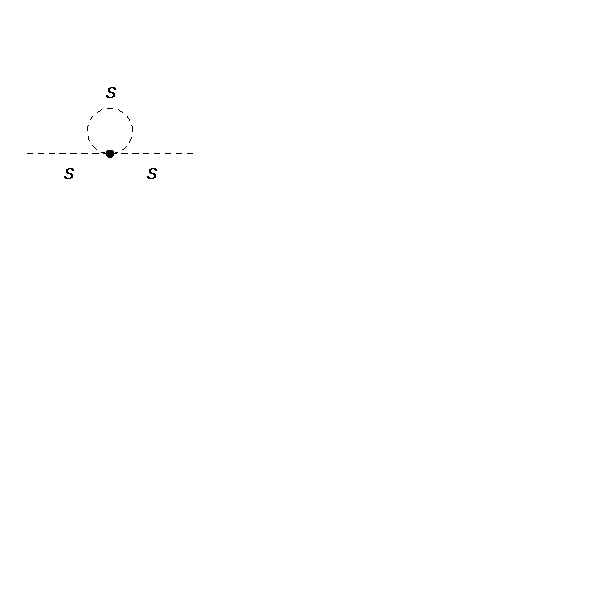
\includegraphics[width=0.8\textwidth]{1loop_1.pdf}\\
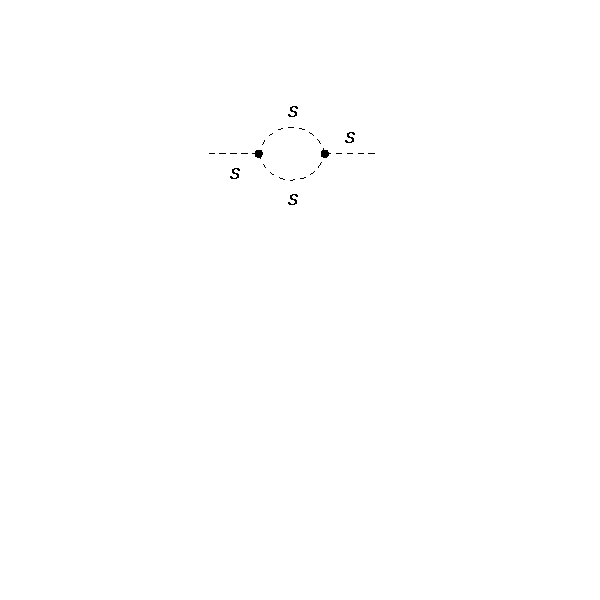
\includegraphics[width=0.8\textwidth]{1loop_2.pdf}\\
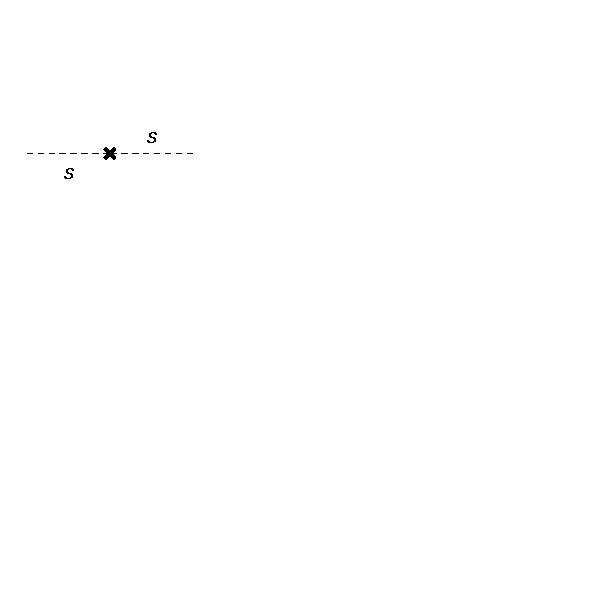
\includegraphics[width=0.8\textwidth]{1loop_c.pdf}
\end{minipage}
\noindent\begin{minipage}{0.7\textwidth}
The ``tadpole" diagram on the left is the easiest to evaluate, the integral is
\begin{align}
\Pi^{(1)}_1 =  \kappa\frac{\lambda}{2} \int \d^4k \frac{-i}{k^2-m^2} =  \kappa \frac{\lambda}{2} \mathbf{A}(m^2)
\end{align}

The result directly from TARCER is
\begin{align}
\Pi^{(1)}_1 = -i \kappa \frac{\lambda}{2} \mathbf{TAI}(m^2)
\end{align}
so after using the relationship $i\mathbf{TAI} = \mathbf{A}$ we see these are equivalent.  The result here is a divergent integral, expressing it as a divergent plus finite piece we have
\begin{align}
\Pi^{(1)}_1 = \frac{1}{2}\kappa\lambda\left(A(m^2)+\epsilon A_{\epsilon}(m^2)-\frac{m^2}{\epsilon}\right).\label{eqn:scalar_1}
\end{align}

\end{minipage}

For the second loop correction we can again quickly write down the integral
\begin{align}
\Pi^{(1)}_2 = -\kappa \frac{g^2}{2} \mathbf{B}(m^2,m^2).
\end{align}
 and then  and $-i\mathbf{TBI} = \mathbf{B}$ to convert to \tsil notation
\begin{align}
\Pi^{(1)}_2 =-i \kappa \frac{g^2}{2} \mathbf{TBI}(m^2,m^2)
\end{align}
which is the output we obtain from TARCER.  The finite plus divergent result is
\begin{align}
\Pi^{(1)}_2 = - \frac{1}{2}\kappa g^2\left(B(m^2)+\epsilon B_{\epsilon}(m^2)+\frac{1}{\epsilon}\right).\label{eqn:scalar_2}
\end{align}
The counter-term diagram is trivial to calculate by hand, yet again we will take the result from \tarcer which is
\begin{align}
\Pi^{(1c)}_1 =  \delta m - \delta Z p^2
\end{align}

We now need to remove the divergent terms from (\ref{eqn:scalar_1}) and (\ref{eqn:scalar_2}) by determining the appropriate values for the counter-term couplings, $\delta m$ and $\delta Z$.  In this case this is a simple calculation, which can do by hand but is also available as a feature in \mb to do automatically.  The full one-loop self energy, including counter-terms, is
 \begin{align}
 \Pi_1 = \frac{1}{2}\kappa\lambda\left(A(m^2)+\epsilon A_{\epsilon}(m^2)-\frac{m^2}{\epsilon}\right)- \frac{1}{2}\kappa g^2\left(B(m^2)+\epsilon B_{\epsilon}(m^2)+\frac{1}{\epsilon}\right)+ \delta m - \delta Z p^2
 \end{align}
where the divergent part is
\begin{align}
\Pi_1^{1/\epsilon}=  -\frac{1}{2\epsilon}\kappa\left(\lambda m^2+g^2\right)+ \delta m - \delta Z p^2
\end{align}
so we find
\begin{eqnarray}
&\delta m &=\frac{\kappa}{2\epsilon} \left(g^2+\lambda m^2\right)+\mathcal{O}(\kappa^2)\\
&\delta Z &= \mathcal{O}(\kappa^2)
\end{eqnarray}
where we allow for high order terms which are required to cancel divergences from amplitudes above the one-loop order.\\

\subsection{Two-loop self energy}

There are 9 loop corrections and 5 counter-term corrections to the scalar propagator at the two-loop level.  We present the results as output by \tarcer and the required conversions to \tsil integrals on a diagram by diagram basis in this section.  For the first diagram we show equivalence with the result as it would be computed by hand and from \mb, which for this diagram is non-trivial.  We show this equivalence at the level of finite integrals.  For the rest we either omit this working or the equivalence is immediately evident, and leave the result as divergent integrals for brevity.

\subsection*{Diagram 1}
\noindent\begin{minipage}{0.3\textwidth}
\begin{center}
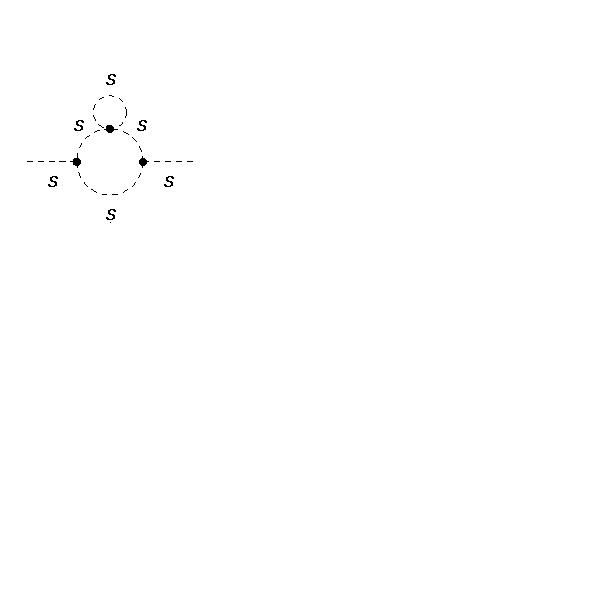
\includegraphics{2loop_1.pdf}\\
\end{center}
\end{minipage}
\noindent\begin{minipage}{0.7\textwidth}
In integral form this diagram can be written down as
\begin{align}
\Pi^{(2)}_1=-\kappa^2\frac{\lambda g^2}{2}\mathbf{A}(x)\mathbf{B}(x',x)\label{eqn:scalar_2a}
\end{align}
using the definitions given in the appendix.  However, we can't deal with derivatives of basis integrals with the computational tools we have as TARCER will always reduce to the most fundamental basis.  So to make a proper check of the tools we must convert this to the most fundamental basis using the relationship
\end{minipage}
\begin{align}
{\bf B}(x',y) = 
\Bigl [ (3-d) (s-x+y) {\bf B}(x,y) + (2-d) \lbrace 
{\bf A}(y) 
+ (s-x-y){\bf A}(x)/2x \rbrace \Bigr ]/\Delta_{sxy} \label{eqn:deltaxyz}
\end{align}
where
\begin{align}
\Delta_{abc} \equiv a^2 + b^2 + c^2 - 2 a b - 2 a c - 2 b c.
\end{align}

Now we will work through from the initial divergent basis integrals in (\ref{eqn:scalar_2a}) and obtain all finite contributions to the amplitude and compare this with the result from \mb.  First I deal with $\mathbf{B}_p(m^2,m^2)$.  From (\ref{eqn:deltaxyz}) setting $x=y$ we have
\begin{align}
\mathbf{B}(x',x) = \frac{2x(3-D)\mathbf{B}(x,x)+(2-D)\mathbf{A}}{2x(s-4x)}
\end{align}
Now we use the relationships $\mathbf{A(x)} = -x/\epsilon +A(x)$ and $\mathbf{B}(x,y) = 1/\epsilon + B(x,y)$, along with setting $D = 4-2\epsilon$ to obtain
\begin{align*}
\Pi &= \frac{\left( -\frac{x}{\epsilon}+A(x)\right)\left[2x(2\epsilon-1)\left( \frac{1}{\epsilon}+B(x,x)\right) + (2\epsilon-2)\left(-\frac{x}{\epsilon}+A(x)\right)\right]}{2x(s-4x)}\\
&= \frac{1}{2x(s-4x)} \left(-2x^2B(x,x)-2A(x)B(x,x)-2(A(x))^2\right)
\end{align*}
So setting $x=m^2$ and $s=p^2$ we have
\begin{align}
\Pi = -\frac{g^2\lambda}{2(16\pi^2)^2} \frac{\left(2m^4B(m^2,m^2)+m^2A(m^2)B(m^2,m^2)+(A(m^2))^2\right)}{m^2(p^2-4m^2)}
\end{align}

Evaluating this diagram with FeynArts, FeynCalc and TARCER via \mb we obtain the finite amplitude
\begin{align}
\Pi = -\frac{g^2\lambda}{(16\pi^2)^2} \frac{ \left(m^2A(m^2)B(m^2,m^2) + 2m^4B(m^2,m^2) + (A(m^2))^2 \right) }{ 2m^2 (4m^2-p^2)}
\end{align}
which agrees with the result computed by hand above.

\subsection*{Diagram 2 and 3}
\noindent\begin{minipage}{0.3\textwidth}
\begin{center}
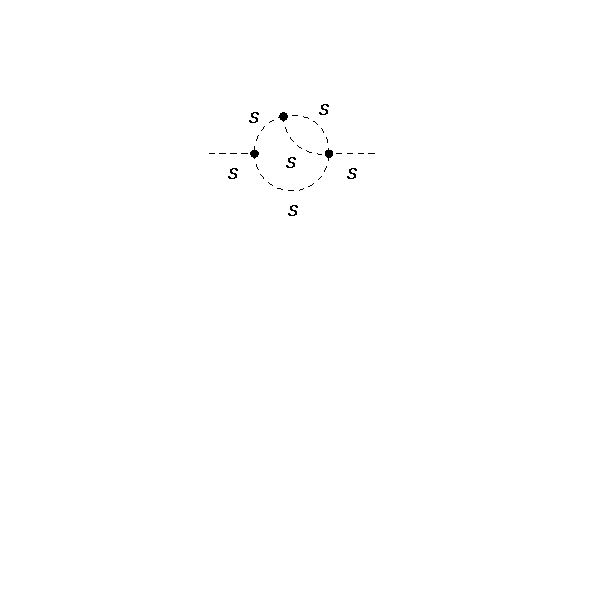
\includegraphics{2loop_2.pdf}\\
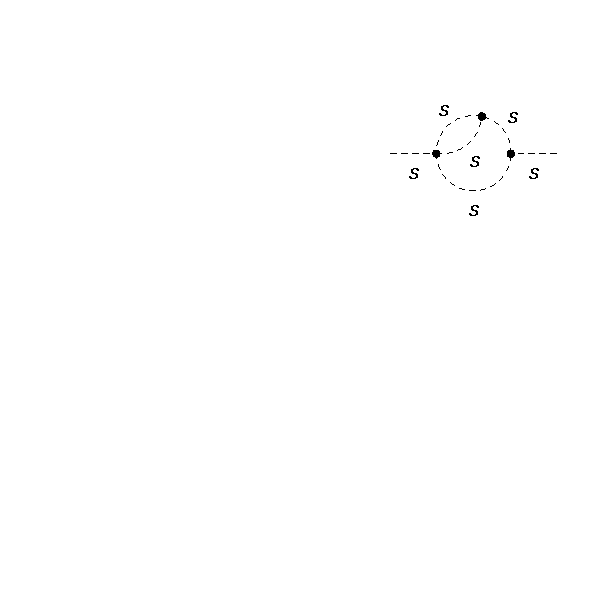
\includegraphics{2loop_3.pdf}\\
\end{center}
\end{minipage}
\noindent\begin{minipage}{0.7\textwidth}
Diagrams 2 and 3 are identical and are given in \tarcer to be
\begin{align}
\Pi_2 = -\kappa^2 \frac{g^2\lambda}{2} \mathbf{TVI}(m^2,m^2,m^2,m^2)
\end{align}
so combining these together and using the result $ \mathbf{TVI}=-\mathbf{U}$ we obtain, the same result as we could get by simply looking at the topology of the diagram
\begin{align}
\Pi_2 =  \kappa^2 g^2\lambda \mathbf{U}(m^2,m^2,m^2,m^2).
\end{align}
\end{minipage}




\subsection*{Diagram 4}

\noindent\begin{minipage}{0.3\textwidth}
\begin{center}
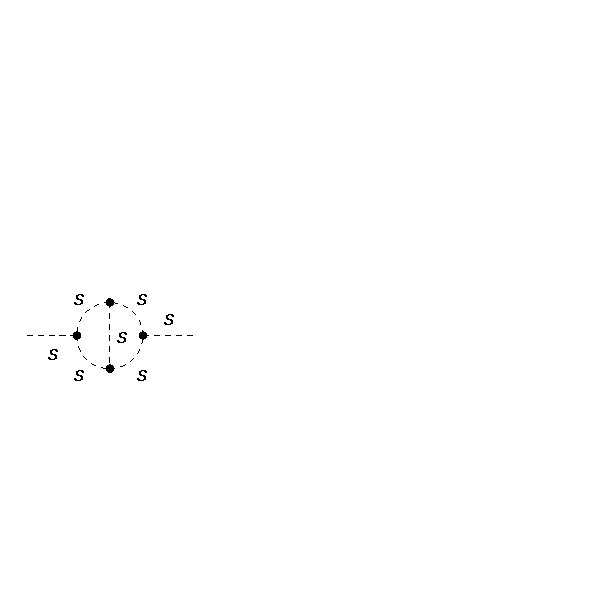
\includegraphics{2loop_4.pdf}
\end{center}
\end{minipage}
\noindent\begin{minipage}{0.7\textwidth}
This diagram represents the ``master" integral which has no divergences and is expressed, in the context of this amplitude, as
\begin{align}
\Pi_4 = -\kappa^2 \frac{g^4}{2} \mathbf{TFI}(m^2,m^2,m^2,m^2,m^2)
\end{align}
making the conversion to \tsil notation, $\mathbf{TFI}=\mathbf{M}$, we have
\begin{align}
\begin{split}
\Pi_4 &= - \kappa^2 \frac{g^4}{2} \mathbf{M}(m^2,m^2,m^2,m^2,m^2)\\&=- \kappa^2 \frac{g^4}{2} M(m^2,m^2,m^2,m^2,m^2)+\mathcal{O}(\epsilon).
\end{split}
\end{align}
\end{minipage}


\subsection*{Diagram 5}
\noindent\begin{minipage}{0.3\textwidth}
\begin{center}
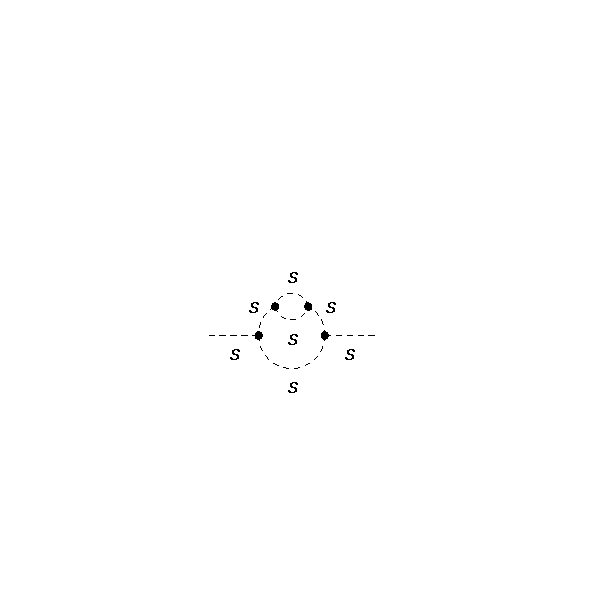
\includegraphics{2loop_5.pdf}



\end{center}
\end{minipage}
\noindent\begin{minipage}{0.7\textwidth}
This diagram is given by TARCER to be, in terms of divergent integrals,
\begin{align}
\begin{split}
\Pi_5 =&- \kappa^2 \frac{g^4}{12 m^4} \left( \frac{3(3D-8)m^2(2m^2-p^2)}{p^2(4m^2-p^2)}\mathbf{TJI}(m^2,m^2,m^2)\right. \\
&+ \frac{4m^2(m^2-p^2)(9m^2-p^2)}{p^2(4m^2-p^2)}\mathbf{TJI}_2(m^2,m^2,m^2)\\
&+\frac{3(D-2)m^2(2m^2-p^2)}{p^2(4m^2-p^2)}\mathbf{TKI}(m^2,m^2,m^2)\\
&+\frac{m^2(D p^2+2(D-9)m^2)}{4m^2-p^2}\mathbf{TVI}(m^2,m^2,m^2,m^2)\\
&\left.+2(D-2)\mathbf{TAI}(m^2) \mathbf{TBI}(m^2,m^2) \right)
\end{split}
\end{align}
\end{minipage}
converting to TSIL notation we obtain

\begin{align}
\begin{split}
\Pi_5 =& - \kappa^2 \frac{g^4}{12 m^4} \left( \frac{3(3D-8)m^2(2m^2-p^2)}{p^2(4m^2-p^2)}\mathbf{S}(m^2,m^2,m^2)\right. \\
&-\frac{4m^2(m^2-p^2)(9m^2-p^2)}{p^2(4m^2-p^2)}\mathbf{T}(m^2,m^2,m^2)\\
&+\frac{3(D-2)m^2(2m^2-p^2)}{p^2(4m^2-p^2)}\mathbf{I}(m^2,m^2,m^2)\\
&-\frac{m^2(D p^2+2(D-9)m^2)}{4m^2-p^2}\mathbf{U}(m^2,m^2,m^2,m^2)\\
&\left.+2(D-2)\mathbf{A}(m^2) \mathbf{B}(m^2,m^2) \right)
\end{split}
\end{align}


\subsection*{Diagram 6}
\noindent\begin{minipage}{0.3\textwidth}
\begin{center}
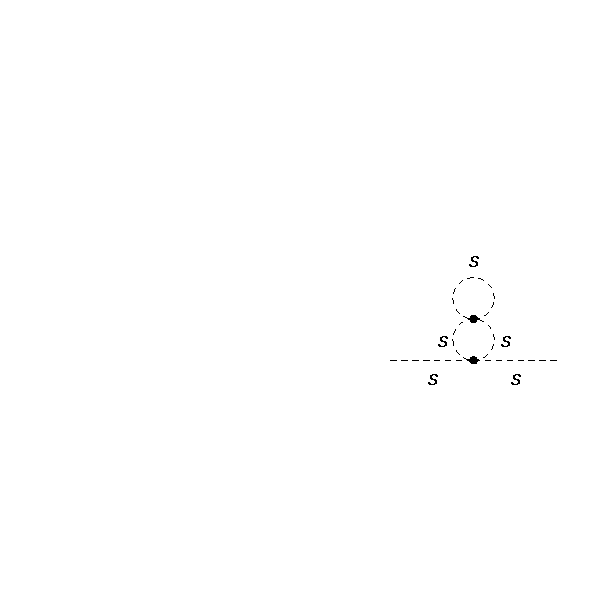
\includegraphics{2loop_6.pdf}
\end{center}
\end{minipage}
\noindent\begin{minipage}{0.7\textwidth}
This diagram is given by TARCER to be
\begin{align}
\Pi_6 &= -\kappa^2 \frac{\lambda^2(D-2)}{8}\frac{ \left({\tt{\mathbf{TAI}}} (m^2)\right)^2}{ m^2 }  
\end{align}
converting to TSIL notation and accounting for the negative sign we obtain
\begin{align}
\Pi_6 &=- \kappa^2 \frac{\lambda^2(D-2)}{8}\frac{ \left({\tt{\mathbf{A}}} (m^2)\right)^2}{ m^2 }  
\end{align}
\end{minipage}

now we must set $D=4-2\epsilon$ and account for finite contributions which come from the divergent parts of the basis integrals.  The basis integrals can be expressed as a finite piece plus a divergent piece, so we have
\begin{align}
{\tt{\mathbf{TAI}}}(x) &= \frac{ix}{\epsilon} +  {\tt{TAI}}(x)
\end{align}
where we have converted \textcolor{blue}{(1.28)} of the TSIL manual into the TARCER definition using $\mathbf{A}= ia \tt{\mathbf{TAI}}$ and taking $a=1$ for small $\epsilon$ (see the \mb manual for the equivalent relationship for all basis integrals).  So the amplitude becomes
\begin{align*}
\Pi_1 &=- \frac{\lambda^2(2-2\epsilon)}{8 m^2 }       \left( {\tt{TAI}}(m^2) +\frac{im^2}{\epsilon}\right)^2  \\
&=- \frac{\lambda^2}{4 m^2 }  {\tt{TAI}}(m^2) \left( \frac{ {\tt{TAI}}(m^2) } {m^2} - 2i\right)
\end{align*}
where we ignore any divergent terms (we will be careful to account for these properly later) and take the limit of $\epsilon\rightarrow 0$.\\

Finally we need to evaluate this in terms of TSIL integrals, which have a different normalization.  The relationship is $\mathbf{A}= ia \tt{\mathbf{TAI}}$ where $a = (4\pi\mu^2)^{2-D/2} \approx 1 +\frac{r\epsilon}{2}\log(4\pi\mu^2)+\mathcal{O}(\epsilon^2)$.  Since we have already removed the divergent parts and are dealing with finite integrals, I take $\epsilon =  0$ and we simply have $\mathbf{A}= i \tt{\mathbf{TAI}}$.  Therefore we end up with
\begin{align}
\Pi_1 & = \kappa^2  \frac{\lambda^2}{4 } A(m^2) \left( \frac{A(m^2)}{m^2} + 2 \right)
\end{align}




\subsection*{Diagram 7}
\noindent\begin{minipage}{0.3\textwidth}
\begin{center}
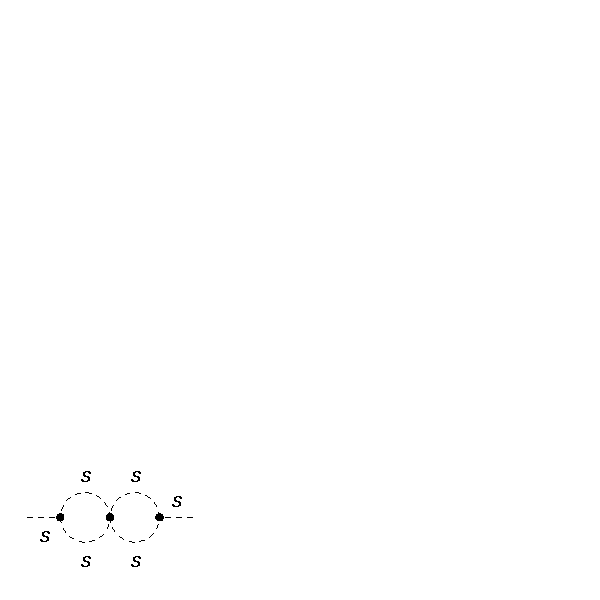
\includegraphics{2loop_7.pdf}
\end{center}
\end{minipage}
\noindent\begin{minipage}{0.7\textwidth}
This diagram is given by TARCER to be
\begin{align}
\Pi_7 & =  -\kappa^2 \frac{g^2 \lambda}{4 } \left(\mathbf{TBI}(m^2,m^2)\right)^2
\end{align}
using $-i\mathbf{TBI}(x,y) = \mathbf{B}(x,y)$ we obtain
\begin{align}
\Pi_7 & = \kappa^2 \frac{g^2 \lambda}{4 } \left(\mathbf{B}(m^2,m^2)\right)^2
\end{align}
\end{minipage}


\subsection*{Diagram 8}
\noindent\begin{minipage}{0.3\textwidth}
\begin{center}
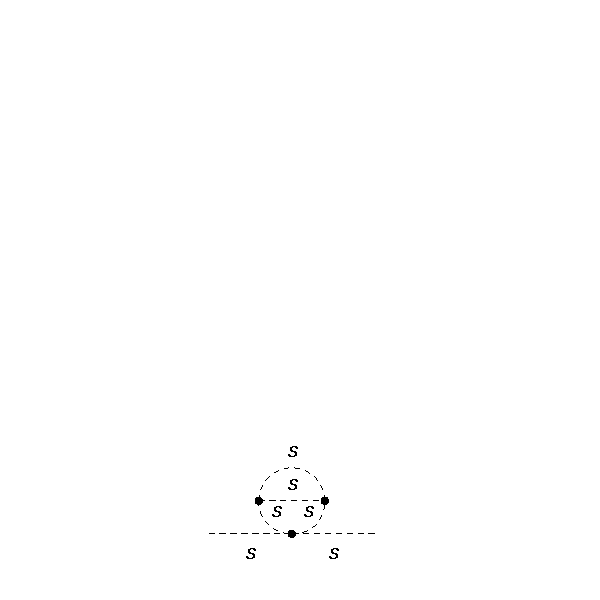
\includegraphics{2loop_8.pdf}
\end{center}
\end{minipage}
\noindent\begin{minipage}{0.7\textwidth}
This diagram is given by TARCER to be
\begin{align}
\Pi_8 & =  \kappa^2\frac{g^2 \lambda}{12 m^2 } (D-3) \mathbf{TKI}(m^2,m^2,m^2)
\end{align}
converting to TSIL notation we obtain and including a relative negative sign for the definition of K 
\begin{align}
\Pi_8 & =  -\kappa^2\frac{g^2 \lambda}{12 m^2 } (D-3) \mathbf{I}(m^2,m^2,m^2).
\end{align}
\end{minipage}

\subsection*{Diagram 9}
\noindent\begin{minipage}{0.3\textwidth}
\begin{center}
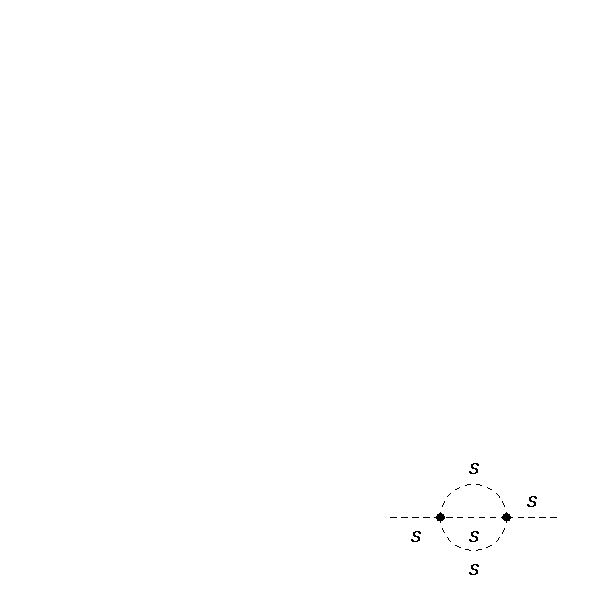
\includegraphics{2loop_9.pdf}
\end{center}
\end{minipage}
\noindent\begin{minipage}{0.7\textwidth}
This diagram is given by TARCER to be

 \begin{align}
 \Pi_9 =\kappa^2 \frac{\lambda^2 {\tt{\mathbf{TJI}}}(m^2,m^2,m^2) }{6}
 \end{align}
 where ${\tt{\mathbf{TJI}}} = {\tt{\mathbf{TJI}}}\{1,1,1\}$ which is equivalent to the TSIL integral $S(x,y,z)$ for $a=1$, accounting for the negative sign we obtain
 \begin{align*}
 \Pi_9 & = -\kappa^2\frac{\lambda^2}{6}\textbf{S}(m^2,m^2,m^2).
 \end{align*}
 \end{minipage}
 
 \subsection*{Counter-diagram 1}
 \noindent\begin{minipage}{0.3\textwidth}
\begin{center}
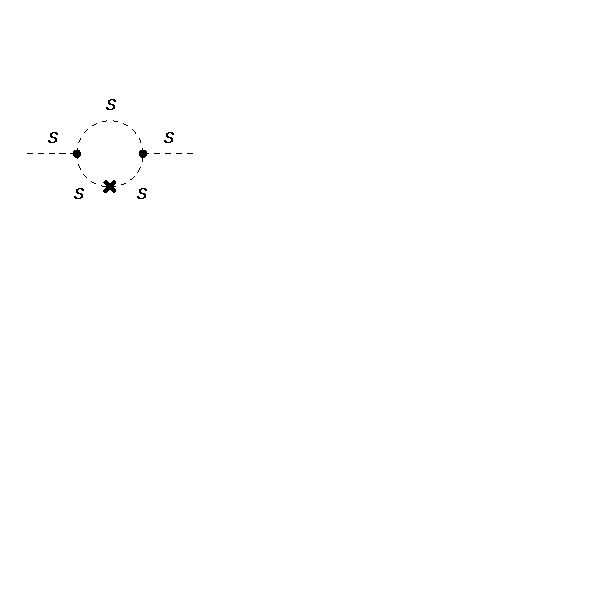
\includegraphics{2loop_1c.pdf}
\end{center}
\end{minipage}
\noindent\begin{minipage}{0.7\textwidth}
The first counter-term diagram involves a correction to the internal scalar propagator and has an amplitude given by TARCER to be
 \begin{align}
 \begin{split}
 \Pi_1 = \kappa\frac{ 1 }{\epsilon} \frac{i  d_1 g^2}{ 2 m^2 (4m^2-p^2)} \left( (D-2){\tt{\mathbf{TAI}}}(m^2)\right.&\\
 \left.-2(D-3){\tt{\mathbf{TBI}}}(m^2,m^2) \right)&
 \end{split}
 \end{align}
  \end{minipage}
where we have also multiplied the computed result by $1/\epsilon$\footnote{We could either include the $1/\epsilon$ in the definition of the counter-term coupling or insert it now, this keep the counter-term coupling as a finite quantity and enables us to identify what the finite terms are before determining the coupling.}.  Converting to \tsil notation we find
  \begin{align}
 \Pi_1 = \kappa \frac{ d_1 }{\epsilon}\frac{g^2}{ 2 m^2 (4m^2-p^2)} \left( (2-2\epsilon){\tt{\mathbf{A}}}(m^2)+2(1-2\epsilon){\tt{\mathbf{B}}}(m^2,m^2) \right)  
 \end{align}
 from which we obtain the finite contribution
 \begin{align}
 \Pi_1 = \kappa d_1 \frac{g^2}{ 2 m^2 (4m^2-p^2)} \left( -2 A(m^2)+2A_{\epsilon}(m^2)-4m^2B(m^2,m^2)+2Bm^2_{\epsilon}(m^2,m^2)\right).
 \end{align}
 
  \subsection*{Counter-diagram 2}
  \noindent\begin{minipage}{0.3\textwidth}
 \begin{center}
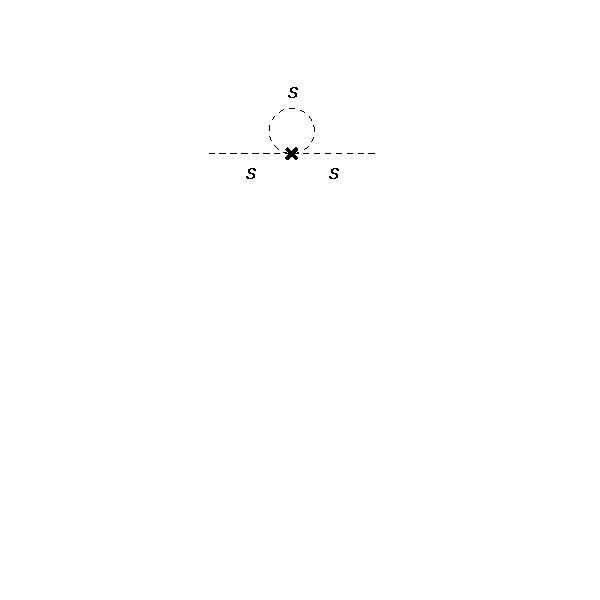
\includegraphics{2loop_2c.pdf}
\end{center}
\end{minipage}
\noindent\begin{minipage}{0.7\textwidth}

 \begin{align}
 \Pi_2 = \frac{ 1 }{\epsilon} \kappa i  \frac{d_{\lambda}}{2} {\tt{\mathbf{TAI}}}(m^2)
 \end{align}
 converting from TARCER to TSIL we obtain
  \begin{align}
 \Pi_2 = - \frac{ 1 }{\epsilon}\kappa \frac{d_{\lambda}}{2} \ {\tt{\mathbf{A}}}(m^2)
 \end{align}
 \end{minipage}
 which given the form of ${\tt{\mathbf{A}}}(m^2)$ contains no finite contributions.  However it is still required to set the value of $d_{\lambda}$ and cancel the divergences from other diagrams.

 
   \subsection*{Counter-diagram 3 and 5}
 \noindent\begin{minipage}{0.3\textwidth}
 \begin{center}
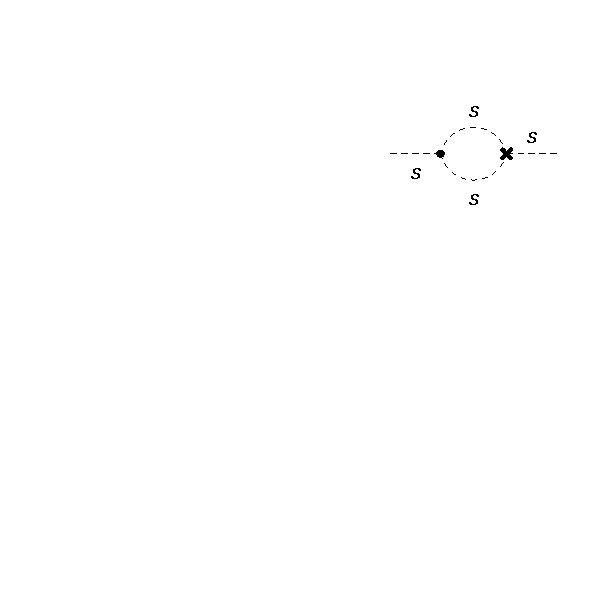
\includegraphics{2loop_3c.pdf} \ \ \ \ \ \ \ 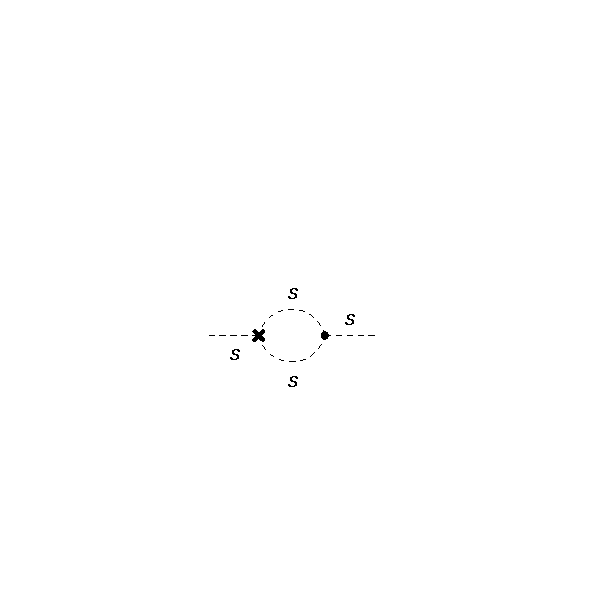
\includegraphics{2loop_5c.pdf}
\end{center}
\end{minipage}
\noindent\begin{minipage}{0.7\textwidth}
Counter-term diagrams 3 and 5 are identical and have a total amplitude of
 \begin{align}
 \Pi_{3,5} = \kappa i \frac{g d_g}{\epsilon} {\tt{\mathbf{TBI}}}(m^2,m^2) 
 \end{align}
converting to TSIL notation and inserting the counter-term coupling (each introduces a negative sign)
\begin{align}
 \Pi_{3,5} = \kappa^2 g \frac{c_{1,1}^g}{\epsilon} {\tt{\mathbf{B}}}(m^2,m^2) 
 \end{align}
\end{minipage}
 
\subsection*{Counter-diagram 4}
\noindent\begin{minipage}{0.3\textwidth}
\begin{center}
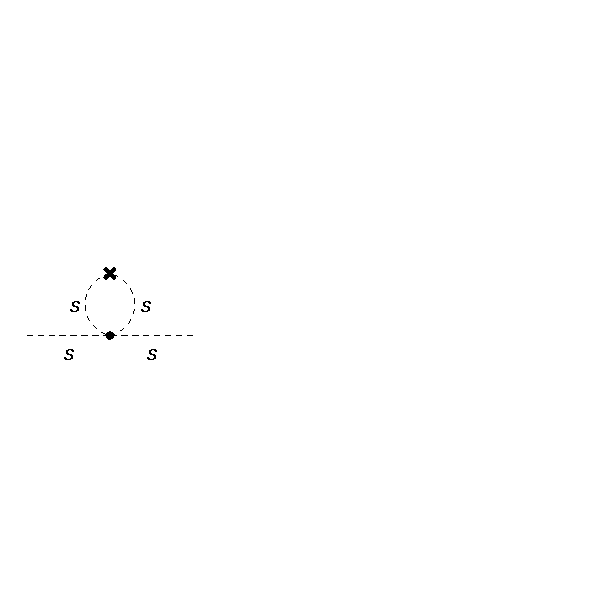
\includegraphics{2loop_4c.pdf}
\end{center}
\end{minipage}
\noindent\begin{minipage}{0.7\textwidth}

 \begin{align}
 \Pi_4 =  \frac{ 1 }{\epsilon}\kappa \frac{i \lambda d_1 (D-2)}{ 4 m^2} {\tt{\mathbf{TAI}}}(m^2) 
 \end{align}
changing to \tsil notation we find
 \begin{align}
 \Pi_4 =  \frac{ 1 }{\epsilon}\kappa \frac{ \lambda d_1 (D-2)}{ 4 m^2} {\tt{\mathbf{A}}}(m^2) 
 \end{align}
 \end{minipage}

\subsection{The counter-term couplings and removing divergences}

The final step is the most non-trivial and involves cancelling all divergences by a careful choice of counter-term couplings.  We use Mathematica to solve a set of simultaneous equations for the counter-term couplings.  There are five counter-terms to determine up to the order in $\epsilon$ we require, the first of these has already been calculated in the first section, leaving four to compute from the full amplitude.\\

If $\Pi=\sum_{i=1}^{2} \Pi^{(1)}_i + \sum_{i=1}^{9} \Pi^{(2)}_i + \Pi^{(1c)}_1 + \sum_{i=1}^{5} \Pi^{(2c)}_i$ is the total self energy then we demand that $\Pi$ has no terms of order one or higher in $1/\epsilon$.  We take the coefficients of $1/\epsilon$, and $1/\epsilon^2$, and then subsequently take the coefficients of the $A(x)$ and $B(x,x)$ terms from each of these to form four seperate equations.  These are sufficient to solve the system and obtain the following counter-terms
\begin{align}
c_{11\lambda}=& \frac{3\lambda^2}{2}\\
c_{11g}=& \frac{3g\lambda}{2}\\
c_{22}=& \frac{1}{8}\left(7g^2\lambda+4\lambda^2m^2\right)\\
c_{21}=& \frac{1}{24}\left(-15g^2\lambda+\lambda^2p^2-6\lambda^2m^2\right)
\end{align}
with these counter-term couplings all divergences are removed.  The resultant self energy is
\begin{eqnarray}
\Pi^{(1)}(s) &=& {1\over2}\lambda A(x) - {1\over2}g^2 B(x,x)\\
\Pi^{(2)}(s) &=& -{1\over2}g^4 M(x,x,x,x,x) 
-{1\over2}g^4V(x,x,x,x) +\lambda g^2U(x,x,x,x)
\nonumber\\
&& -{1\over6}\lambda^2 S(x,x,x)
+{1\over4}\lambda g^2 B(x,x)B(x,x)
+{1\over4}\lambda^2 A(x)\left[A(x)/x+1\right]\\
&& - {1\over2}\lambda g^2 A(x)B(x^\prime,x)
- {1\over4}\lambda g^2 I(x^\prime,x,x)\; ,
\nonumber
\end{eqnarray}
where $x=m^2$.



% \section*{Comments}
% 
% In Stephen's working the $A_{\epsilon}(x')$ terms cancel between the diagrams and the counter-term diagrams.  However,
% 
% \begin{align*}
% A_{\epsilon}(x') = \frac{A_{\epsilon}(x)}{x}-\frac{A(x)}{x}
% \end{align*}
% 
% so there is actually a $A(x)$ term here that is cancelling out between the normal diagrams and the finite contribution from the counter-terms, but it's kind of hidden.  In our approach, we do not invoke this derivative at all (and don't carry around non-expanded things like  $A_{\epsilon}(x')$ ) , and thus our diagram (diagram 5) explicitly contains this $A(x)$ term, so it appears wrong until we actually consider the counter-term.  In Stephen's approach we could actually just ignore the  $A_{\epsilon}(x')$  term from the beginning knowing it will cancel.  All this only becomes apparent when we expand out  $A_{\epsilon}(x')$ and look at the counter-term and normal diagrams separately.
 
 



\section{The electroweak triplet model}
\subsection{Introduction}

The extension of the standard model by an electroweak multiplet is a popular dark matter candidate theory.  At the lowest order in perturbation theory all components of the multiplet have the same mass, which would result in charged dark matter, contrary to what is observed.  However when one goes to the next order in perturbation theory by computing the radiatively corrected mass, then the charged component(s) will obtain a slightly larger mass correction than the neutral component, resulting in a sufficient mass splitting to render the charged components to have a lifetime much shorter than the age of the universe.  The exact value of this mass splitting at the two-loop level is of interest.  We will work with the most simple multiplet, a triplet, to determine the value of this mass splitting at the two-loop order in perturbation theory.\\

To further reduce the number of interactions we need to consider we will use a simplified standard model with the most minimal components to achieve a mass splitting.  This model consists of the $U(1)$ and $SU(2)$ gauge sectors but no SM fermions or leptons.  The particle content of the model is given in Table \ref{tab:particles}.  The triplet sector of the Lagrangian is
\begin{align}
\begin{split}
\mathcal{L}_{\chi}=&\frac{1}{2}\overline{\mychi^0}(i\slashed{\partial}-M)\mychi^0+\frac{1}{2}\overline{\mychi^+}(i\slashed{\partial}-M)\mychi^{+}\\
&+g\left(\overline{\mychi^+}\gamma_{\mu}\mychi^+\right)\left(s_wA_{\mu}+c_wZ_{\mu}\right)\\
&+g\left(\overline{\mychi^+}\gamma_{\mu}\mychi^0 \right)W_{\mu}^++\text{h.c.}
\end{split}
\end{align}
where $s_W=\sin(\theta_W)$ and $c_W=\cos(\theta_W)$ are the sine and cosine of the Weinberg angle respectively.

The Higgs sector is given by
\begin{align}
\mathcal{L}_{H}&=\mu^2 \overline{H}H-\lambda(\overline{H}H)^2
\end{align}

The mixing in the gauge sector after EWSB is given by
\begin{align} 
\left(\begin{array}{c} 
B_{{\rho}}\\ 
W_{{3 \rho}}\end{array} \right) 
 = & \,Z^{\gamma Z}
\left(\begin{array}{c} 
\gamma_{{\rho}}\\ 
Z_{{\rho}}\end{array} \right) \\ 
\left(\begin{array}{c} 
W_{{1 \rho}}\\ 
W_{{2 \rho}}\end{array} \right) 
 = & \,Z^{W}
\left(\begin{array}{c} 
W^+_{{\rho}}\\ 
W^+_{{\rho}}\end{array} \right) \\ 
\end{align} 
where the mixing matrices are parametrised by \\ 
\begin{align} 
Z^{\gamma Z}= \, \left( 
\begin{array}{cc} 
c_W  & - s_W   \\ 
 s_W  & c_W \end{array} 
\right) \\ 
Z^{W}= \,\frac{1}{\sqrt{2}}  \left( 
\begin{array}{cc} 
1& 1 \\ 
 i   & -i  \end{array} 
\right). \\ 
\end{align} 

The gauge fixing sector has Lagrangian in the gauge eigenstate
\begin{align} 
L_{GF} = \, &-\frac{1}{2} |\partial_{\mu}B|^2 \xi_{B}^{-1}  -\frac{1}{2} |\partial_{\mu}W|^2 \xi_{W}^{-1} 
\end{align} 
and in the EWSB eigenstate
\begin{align} 
L_{GF} = \, & -\frac{1}{2} A^0 v \xi_{Z} \Big(g_1 \sin\Theta_W   + g_2 \cos\Theta_W  \Big) + \partial_{\mu}Z|^2 \xi_{Z}^{-1}  -\frac{1}{2} |\partial_{\mu}\gamma|^2 \xi_{\gamma}^{-1} \\&-\frac{i}{2} g_2 H^+ v \xi_{W^+}  + \partial_{\mu}W^+|^2 \xi_{W^+}^{-1}.
\end{align} 
In our choice of gauge the ghost fields take on the same mass as their respective field, such that $m_{\eta_{\gamma}} = m_{\gamma}$, $m_{\eta_Z}=m_{Z}$, $m_{\eta^+}=m_{W}$.  The fields $A_0$ and $H^+$ from the pre-EWSB theory are also given the respective masses of $m_{A_0}=m_Z$ and $m_{H^+}=m_W$.

We use the following relationships in the input to \mb, to reduce the number of free variables required at run time
\begin{eqnarray}
\begin{split}
s_w^2&=\frac{g_1^2}{g_1^2+g_2^2}, \ \ \ c_w^2&=\frac{g_2^2}{g_1^2+g_2^2}\\
\alpha&=\frac{g_1^2g_2^2}{g_1^2+g_2^2}, \ \ \ v&=\frac{2m_w}{g_2} \ \ \ \ \alpha=e^2
\end{split}
\end{eqnarray}


\begin{table}[h]
 \caption{The particle content of the electroweak triplet model.}\label{tab:particles}
 \vspace{0.3cm}
 \centering 
\begin{tabular}{lccccc}
\hline 
Name & Type & complex/real & Mass  \\ 
\hline \hline 
\(H^+\) & Scalar &complex& $m_W$\\
 \(A^0\) & Scalar &real & $m_Z$\\
 \(h\) & Scalar &real & $m_H$\\
 \hline 
\(\chi^{+}\) & Fermion &Dirac & $M$\\
 \(\chi_0\) & Fermion &Majorana & $M$\\
 \hline 
\(\gamma\) & Vector &real & $m_{\gamma}$\\
 \(Z\) & Vector &real & $m_Z$\\
 \(W^+\) & Vector &complex & $m_W$\\
 \(\eta^{\gamma}\) & Ghost &real & $m_{\gamma}$\\
 \(\eta^Z\) & Ghost &real & $m_Z$\\
 \(\eta^+\) & Ghost &complex & $m_W$\\
 \(\eta^-\) & Ghost &complex & $m_W$\\
 \hline
\end{tabular}
 \end{table}
The momentum dependent contribution to the triplet mass, the self energy, is given by calculating the 1PI loop process.  For the $
\chi^0$ at one loop level this involves a loop with a W boson and $\chi^{\pm}$ particle, for $\chi^{\pm}$ we also have loops involving $
\chi^{\pm\pm}$, $W^{\pm}$ and the $A$ and $Z$ bosons.  The propagators we will use are (in the Feynman gauge)
\begin{align}
i\Pi^{V}_{\mu\nu}&=-i\frac{-g_{\mu\nu}}{k^2-m_{\text{V}}^2- \Pi(k^2)}\label{eqn:gauge_boson_propagator}\\ 
i\Pi^{\chi}_{\mu\nu}&=-i\frac{\slashed{k}-m}{k^2-m^2- \Pi(k^2)}
\end{align}
for the vector bosons ($V\in\{W^{\pm},\gamma,Z\}$) and the components of the fermionic triplet ($\chi\in\{\chi^0,\chi^{\pm}\}$).\\

The aim of this section is to the compute the full two-loop self energy of the charged and neutral components of the electroweak triplet, $\chi$.  For this we will require the one-loop self energy, the derivative of the one-loop self energy and the two-loop self energy.  To obtain the necessary contributions from the two-loop order counter-terms we will also require the counter-term couplings involved.  For this theory, these are limited to the tree-level counter-term couplings for the gauge bosons and the triplet, along with a single vertex correction.  All these quantities will be presented in the remainder of this section.


\subsubsection{Pole mass calculation}

We present here a detailed discussion of the method of pole mass calculation in the electroweak triplet theory.

The pole mass is obtained from the 1PI effective two-point function,
\begin{equation}
\Gamma_2=\slashed{p}-M_0+\Sigma_K(p^2)\slashed{p}+\Sigma_M(p^2) \label{eqn:propagator}
\end{equation}
where $p$ is the four momentum of the particle and $M_0$ is the tree-level (or MS-bar after renormalisation) mass, and $\Sigma(p^2)=\Sigma_M(p^2)+\slashed{p}\Sigma_K(p^2)$ is the self energy.  We calculate self energies both by hand and using FeynCalc \cite{Mertig1991,Shtabovenko2016} at the one-loop level.  The pole mass is obtained by demanding $\Gamma_2=0$ which can be achieved by setting $p=\slashed{p}=\Mp$ and iterating
\begin{align}
\Mp=\text{Re}\left[\frac{M_0-\Sigma_M(\Mp^2)}{1+\Sigma_K(\Mp^2)}\right]. \label{eqn:M_pole_iterative}
\end{align}

This is the first of two methods to calculate the pole mass, which we will refer to as $\Mpa$ or the \textit{implicit pole mass}.

Alternatively (\ref{eqn:M_pole_iterative}) can be expanded as a power series in the gauge coupling $g$, where for each self energy function we have $\mathcal{O}(\Sigma^{(n)})=\mathcal{O}(g^{2n})$ where $n$ is the number of radiative loop corrections computed for the self energy function.  First, expressing the self energies as a power series in $g$ we have
\begin{align}
\Mp=\text{Re}\left[\frac{M_0-\Sigma^{(1)}_M(\Mp^2)-\Sigma^{(2)}_M(\Mp^2)+\mathcal{O}(g^6)}{1+\Sigma^{(1)}_K(\Mp^2)+\Sigma^{(2)}_K(\Mp^2)+\mathcal{O}(g^6)}\right] \label{eqn:M_pole_1}
\end{align}
Then using a Taylor expansion we find to order $g^6$
\begin{align*}
\begin{split}
\Mp=M_0-\Sigma^{(1)}_M-\Sigma^{(2)}_M-M_0\Sigma^{(1)}_K+\Sigma^{(1)}_M\Sigma^{(1)}_K\ \ \ \ \ \ \ \ \ \ \  \ \ &\\ \left.-M_0\Sigma^{(2)}_K+\Sigma^{(1)}_K\Sigma^{(1)}_K+\mathcal{O}(g^6)\right|_{p^2=\Mp^2}&
\end{split}
\end{align*}
where $\Sigma^{(n)}_X=\Sigma^{(n)}_X(p^2)$ such that $p^2$ is the first argument in the two point functions appearing in the self energies. However, this is still an iterative expression, to get an expression without iterating we must change $p$ here from $\Mp$ to $M_0$.

%\begin{align*}
%\frac{1}{1+x}=1-x+x^2+\mathcal{O}(x^3)
%\end{align*}
%\begin{align*}
%&\left.\frac{1}{1+\Sigma^{(1)}_K+\Sigma^{(2)}_K}\right|_{p=\Mp^2}=\\ &\left.1-\Sigma^{(1)}_K-\Sigma^{(2)}_K+\Sigma^{(1)}_K\Sigma^{(1)}_K+\mathcal{O}(g^6)\right|_{p^2=\Mp^2}
%\end{align*}

Demanding that the self energies are evaluated at the tree level mass requires the use of the Taylor expansion,
%\begin{align}
%f(x^2)=f(a^2)+\left.2x\frac{\d f(x^2)}{\d x^2}\right|_{x=a}(x-a)+\mathcal{O}\left((x-a)^2\right)
%\end{align}
%such that\footnote{This derivation can be done slightly differently, one may apply the following Taylor series to the full self energy (not separated into loop orders), before taking the above series expansion.  However, the end result %is the same if one is consistent with the order of the calculation throughout.}
\begin{align}
\begin{split}
&\left.\Sigma^{(1)}_M\right|_{p^2=\Mp^2}=\\&\left.\Sigma^{(1)}_M+2M_0(\Mp-M_0)\dot{\Sigma}^{(1)}_M+\mathcal{O}\left(g^6\right)\right|_{p^2=M_0^2}. \label{eqn:Taylor_expansion1}
\end{split}
\end{align}
However this is not yet an explicit expression for $\Mp$, so we use the relation
\begin{align}
\begin{split}
\Mp-M_0&=-\Mp\Sigma^{(1)}_K(\Mp^2)-\Sigma^{(1)}_M(\Mp^2)+\mathcal{O}(g^4)\\
&=-\Mp\Sigma^{(1)}_K(M_0)-\Sigma^{(1)}_M(M_0)+\mathcal{O}(g^4)\label{eqn:mass_diff}
\end{split}
\end{align}
which comes directly from demanding  (\ref{eqn:propagator}) be equal to zero, and the second line follows from using (\ref{eqn:Taylor_expansion1}) to discard higher order terms.  An error of order $g^4$ is acceptable for this difference since it appears in the final expression as the coefficient of the term $\dot{\Sigma}^{(1)}_K$ and thus will be a total error of order $g^6$.  Finally, to remove the $\Mp$ on the right-hand side we use the same expression within itself (effectively iterating)
\begin{align}
\begin{split}
\Mp-M_0&=-\Mp\Sigma^{(1)}_K(M_0)-\Sigma^{(1)}_M(M_0)+\mathcal{O}(g^4)\\
%&=-(M_0-\Mp\Sigma^{(1)}_K(M_0)-\Sigma^{(1)}_M(M_0))\Sigma^{(1)}_K(M_0)-\Sigma^{(1)}_M(M_0)+\mathcal{O}(g^4)\\
&=-M_0\Sigma^{(1)}_K(M_0)-\Sigma^{(1)}_M(M_0)+\mathcal{O}(g^4)\label{eqn:M0Mp}\\
\end{split}
\end{align}
substituting this result into (\ref{eqn:Taylor_expansion1}) gives
\begin{align}
\begin{split}
&\left.\Sigma^{(1)}_M\right|_{p^2=\Mp^2}=\\ &\left.\Sigma^{(1)}_M-2M_0(M_0\Sigma^{(1)}_K+\Sigma^{(1)}_M)\dot{\Sigma}^{(1)}_M+\mathcal{O}\left(g^6\right)\right|_{p^2=M_0^2}.
\end{split}
\end{align}


For the two loop corrections we need not compute the details of the derivative term, since we already know it will be above order $g^6$ so we simply use
\begin{align*}
\left.\Sigma^{(2)}_M\right|_{p^2=\Mp^2}=\left.\Sigma^{(2)}_M+\mathcal{O}\left(g^4(\Mp-M_0)^2\right)\right|_{p^2=M_0^2}.
\end{align*}
Similar relations hold for $\Sigma^{(1)}_K$ and $\Sigma^{(2)}_K$.\\

With the use of these expressions we can express (\ref{eqn:M_pole_1}) with all functions evaluated at $M_0$ to give
\begin{align}
\begin{split}
&\Mp=\left[M_0-\Sigma^{(1)}_M-\Sigma^{(2)}_M-M_0\Sigma^{(1)}_K-M_0\Sigma^{(2)}_K\right.\\
&+(\Sigma^{(1)}_M+M_0\Sigma^{(1)}_K)(\Sigma^{(1)}_K+2M_0\dot{\Sigma}^{(1)}_M+2M_0^2\dot{\Sigma}^{(1)}_K)\\
&\left.+\mathcal{O}\left(g^6\right)\right]_{p^2=M_0^2} \label{eqn:M_pole_explicit}
\end{split}
\end{align}
which agrees with Ibe and Sato \cite{Ibe2013a}.  Reducing this to the one-loop level we obtain
\begin{align}
\begin{split}
\Mp&=\left[M_0-\Sigma^{(1)}_M-M_0\Sigma^{(1)}_K+\mathcal{O}\left(g^4\right)\right]_{p^2=M_0^2} \label{eqn:M_pole_explicit_1_loop}
\end{split}
\end{align}
which is the second method of pole mass calculation we will use, we refer to this as $\Mpb$ or the \textit{explicit pole mass}.

In summary, we have derived an explicit expression for the pole mass by invoking the perturbativity of the gauge coupling.  The purpose for doing so is that (\ref{eqn:M_pole_explicit_1_loop}) makes it possible to derive an expression for the mass splitting as one may simply take the difference of this expression for each quintuplet component.  Such a procedure is not possible with the pole mass implicitly defined in (\ref{eqn:M_pole_iterative}), instead one must iterate until convergence is achieved, and then take the difference of the numerical results.



\subsection{One-loop self energy -- neutral component}
\noindent\begin{minipage}{0.3\textwidth}
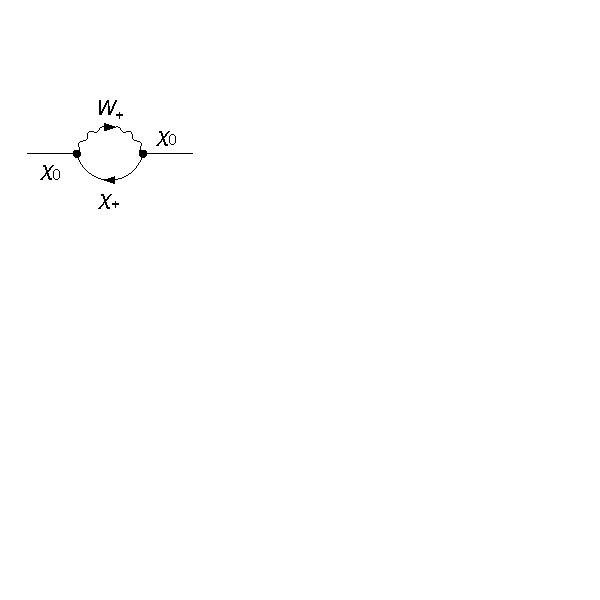
\includegraphics[width=0.8\textwidth]{1loop_a.pdf}\\
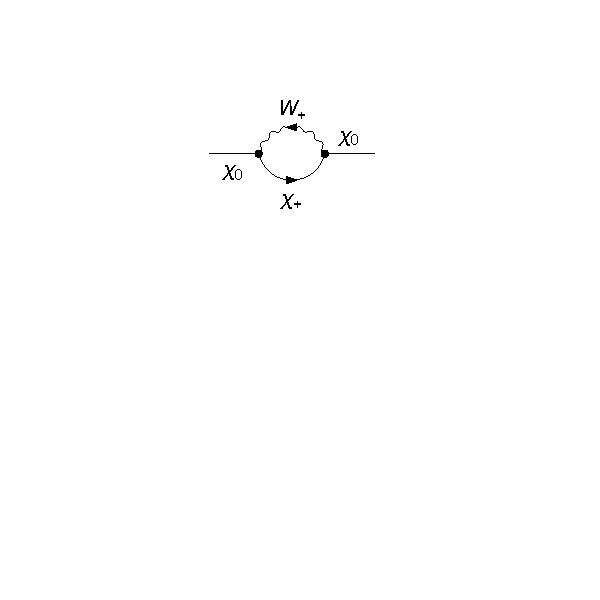
\includegraphics[width=0.8\textwidth]{1loop_b.pdf}
\end{minipage}
\noindent\begin{minipage}{0.7\textwidth}

The neutral component only has two possible radiative corrections, due to the processes $\chi_0\rightarrow W^{\pm} + \chi^{\mp}$.  The corresponding Feynman diagrams are given on the left.  The loop integral we need to evaluate is
\begin{align}
i\Sigma_{\cn}(\slashed{p})&= 2 (-gi)^2 \int \frac{\d^4k}{(2\pi)^4} \gamma^{\mu}\frac{(\slashed{p}-\slashed{k}+m)\gamma^{\nu}\left(-g_{\mu\nu}\right)}{((p-k)^2-m^2)(k^2-m_{\text{w}}^2)}\label{eqn:cn_loop}
\end{align}
where we have included a factor of two since this process can occur via either $\chi_0\rightarrow W^+ + \chi^-$ or $\chi_0\rightarrow W^- + \chi^+$.  
\end{minipage}

We will calculate the neutral component self energy by hand and confirm that it is consistent with that given by FeynCalc to verify both the tools and our input model.  The loop integral is expressed as
\begin{align}
i\Sigma_{\cn}(\slashed{p})&= (-gi)^2 \int \frac{\d^4k}{(2\pi)^4} \frac{N}{((p+k)^2-m^2)(k^2-m_{\text{w}}^2)}
\end{align}
where we simplify $N$ by
\begin{align*}
N&=-\gm(\sk+\sp+m)\gn g_{\mu\nu}\\
&=-\gm(\sk+\sp+m)\gamma_{\mu}\\
&=2(\sk+\sp)-4m
\end{align*}

using the identities
\begin{align}
\begin{split}
\gamma_{\mu}\slashed{a}\gm&=-2\slashed{a}\\
\gm\gamma_{\mu}&=4I_4
\end{split}
\end{align}
where $I_4$ is the identity matrix in 4 dimensions.

Now we use the Feynman parameter integral
\begin{align}
\frac{1}{AB}=\int_0^1 \frac{\d x}{[A+(B-A)x]^2}
\end{align}
to simplify the denominator
\begin{align*}
 \frac{1}{((p-k)^2-m^2)(k^2-m_{\text{w}}^2)}&=\int_0^1\frac{\d x}{[k^2-m_{\text{w}}^2+(p^2-2kp+k^2-(k^2-m_{\text{w}}^2))x]^2}\\
&=\int_0^1\frac{\d x}{[ k^2-2kpx+p^2x+x(m_{\text{w}}^2-m^2)-m_{\text{w}}^2]^2}\\
&=\int_0^1\frac{\d x}{[ (k-px)^2+x(1-x)p^2+x(m_{\text{w}}^2-m^2)-m_{\text{w}}^2]^2}\\
&=\int_0^1\frac{\d x}{[ k'-\Delta]^2}
\end{align*}
where $k'=k-px$ and $\Delta=-x(1-x)p^2-x(m_{\text{w}}^2-m^2)+m_{\text{w}}^2$.


We now translate the integration measure $\int \d^4k\rightarrow\int \d^4k'$ (and henceforth omitting the prime on $k'$) to obtain (after substituting $k\rightarrow k+px$ in the numerator)
\begin{align}
i\Sigma_{\cn}(\slashed{p})&= (-gi)^2 \int \frac{\d^4k}{(2\pi)^4}\int_0^1 \d x \frac{2(\sp(1-x)-\sk )-4m}{[ k^2-\Delta]^2}
\end{align}
after shifting the integration measure.

since the denominator of the loop integral is symmetric with respect to $k$ we can discard all terms here of odd order in $k$, thus
\begin{align}
i\Sigma_{\cn}(\slashed{p})&= (-gi)^2 \int \frac{\d^4k}{(2\pi)^4}\int_0^1 \d x \frac{2(\sp(1-x))-4m}{[ k^2-\Delta]^2}
\end{align}



Now we apply dimensional regularisation, letting $d=4-\epsilon$, such that in the limit of small $\epsilon$ we have


\begin{align*}
\int \frac{\d^4k}{(2\pi)^4}{[ k^2-\Delta]^2} &\rightarrow  \mu^{\epsilon}\int \frac{\d^dk}{(2\pi)^d}  \frac{1}{[ k^2-\Delta]^2}\\
&= \mu^{\epsilon}\frac{i}{(4\pi)^{\frac{d}{2}}} \frac{1}{\Delta^{2-\frac{d}{2}}} \Gamma\left(\frac{4-d}{2}\right) \\
&= \mu^{\epsilon}\frac{-i}{(4\pi)^2}\frac{1}{\Delta^{\epsilon/2}}\Gamma\left(\frac{\epsilon}{2}\right) (4\pi)^{\epsilon/2}\\
&\approx \frac{i}{(4\pi)^2} \left( 1-\he\log\Delta\right)\left(\frac{2}{\epsilon}-\gamma\right)\left(1+\he\log 4\pi\right)\left(1+\he\log\mu^2\right)\\
&=\frac{i}{(4\pi)^2} \left(\frac{2}{\epsilon}-\gamma+\log\frac{4\pi\mu^2}{\Delta}\right)+\mathcal{O}(\epsilon)
\end{align*}

We are now ready to calculate the integral for $i\Sigma_{\cn}(\slashed{p})$.

\begin{align}
i\Sigma_{\cn}(\slashed{p})&= (-gi)^2 \frac{i}{(4\pi)^2}  \int_0^1 \d x \left(2(\sp(1-x))-4m\right) \left(\frac{2}{\epsilon}+\log\frac{\hat{\mu}^2}{\Delta}\right)
\end{align}
where $\hat{\mu}^2=4\pi\mu^2e^{-\gamma}$.

The Passarino-Veltman functions we have are (from arXiv:1212.5989)
\begin{align}
B_0(p^2,m_1^2,m_2^2)&=\int_0^1\!\d x \ \log\frac{\hat{\mu}}{\Delta}\\
B_1(p^2,m_1^2,m_2^2)&=-\int_0^1\!\d x \ x\log\frac{\hat{\mu}}{\Delta}
%B_{21}(p^2,m_1^2,m_2^2)&=\int_0^1\!\d x \ x^2\log\frac{\hat{\mu}}{\Delta}
\end{align}
\textcolor{red}{FIX THIS TO MATCH TSIL NOTATION AND DISCUSS DIVERGENT TERMS}
\begin{align}
i\Sigma_{\cn}(\slashed{p})&= (-gi)^2 \frac{i}{(4\pi)^2}  \left(2\sp\left( B_0(p^2,m_{\text{w}}^2,m^2)+B_1(p^2,m_{\text{w}}^2,m^2)\right)-4mB_0(p^2,m_{\text{w}}^2,m^2)\right)
\end{align}

To bring it into the same form as given by FeynCalc we use the identity $B_1(p^2,m_1^2,m_2^2)=-B_1(p^2,m_2^2,m_1^2)-B_0(p^2,m_2^2,m_1^2)$ such that
\begin{align}
\Sigma_{\cn}(m)&= \frac{2mg^2}{(4\pi)^2}   \left( 2B_0(p^2,m^2,m_{\text{w}}^2)+B_1(p^2,m^2,m_{\text{w}}^2)\right)
\end{align}


\noindent\begin{minipage}{0.3\textwidth}
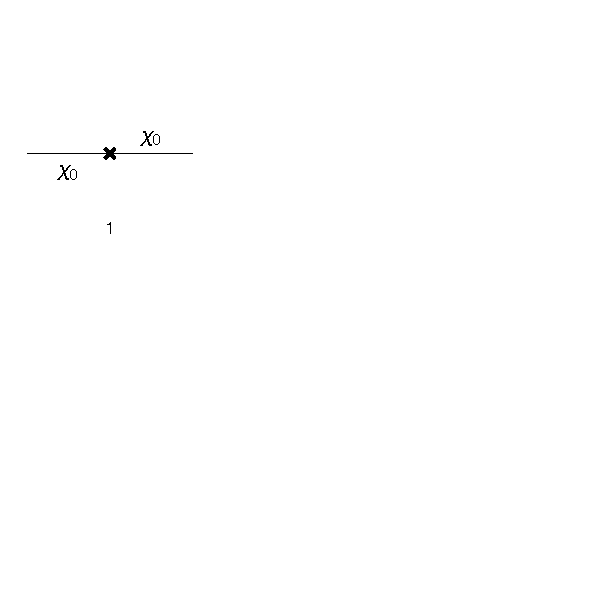
\includegraphics[width=0.8\textwidth]{1loop_1c.pdf}
\end{minipage}
\noindent\begin{minipage}{0.7\textwidth}
There is also a counter-term contribution, with amplitude
\begin{align}
 \int \frac{\d^4k}{(2\pi)^4} \delta_{M_{\tilde{\chi}}} + \slashed{p}\delta_{Z_{\tilde{\chi}}}
 \end{align}
 \end{minipage}

Evaluating these amplitudes gives the self energy $\Sigma_{\cn}= \Sigma_{M, 0}^{(1)}+\slashed{p}\Sigma_{K, 0}^{(1)}$ where
\begin{eqnarray}
\Sigma_{K, 0}^{(1)} &=&
-\frac{\hat{g}^2}{16\pi^2}
\left[ 4 B_1(p^2, \hat{M}_2^2, \hat{m}_W^2) + 2 \right]
+\delta_{Z_{\tilde{\chi}}}\ , \label{eq: Neu_K} \\
%%%%%
\Sigma_{M, 0}^{(1)} &=&
-\frac{\hat{g}^2 \hat{M}_2}{16\pi^2}
\left[ 8 B_0(p^2, \hat{M}_2^2, \hat{m}_W^2) - 4 \right]
-\delta_{M_{\tilde{\chi}}}\ . \label{eq: Neu_M}
\end{eqnarray}


\subsection{One-loop self energy -- charged component}

\noindent\begin{minipage}{0.3\textwidth}
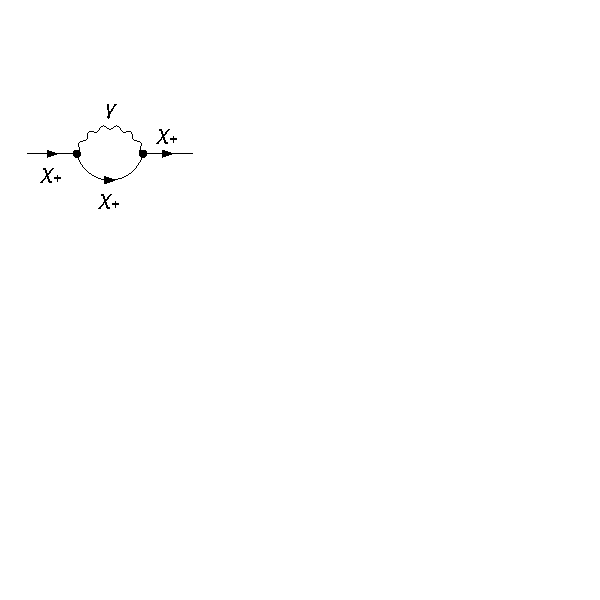
\includegraphics[width=0.8\textwidth]{F1_1_a.pdf}\\
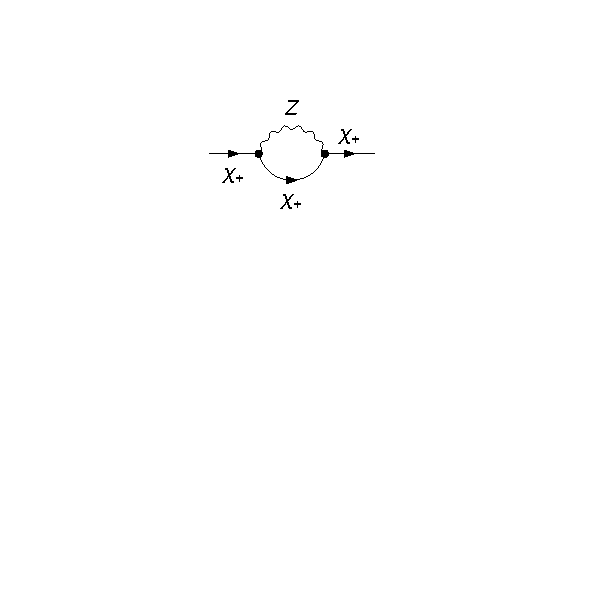
\includegraphics[width=0.8\textwidth]{F1_1_b.pdf}\\
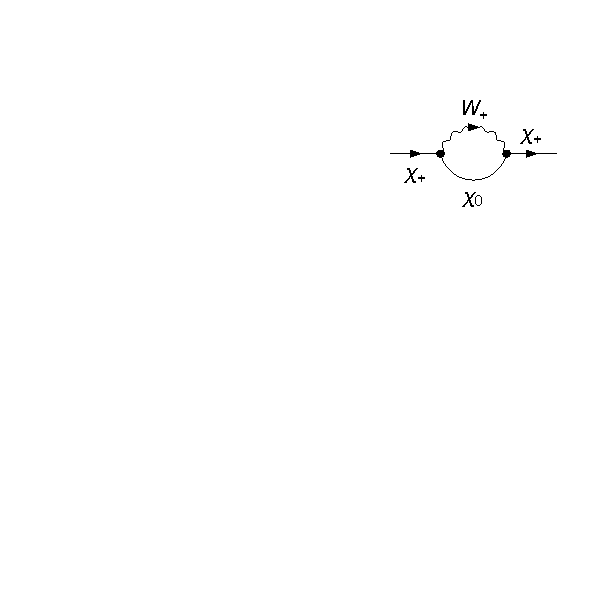
\includegraphics[width=0.8\textwidth]{F1_1_c.pdf}
\end{minipage}
\noindent\begin{minipage}{0.7\textwidth}

The charged component has three one-loop corrections with diagrams given on the left.  The total amplitude for all three contributions is
\begin{align}
\begin{split}
i\Sigma_{\cm}(\slashed{p})=
&+(-is_wg)^2 \int \frac{\d^4k}{(2\pi)^4} \gamma^{\mu}\frac{(\slashed{p}-\slashed{k}+M)\gamma^{\nu}\left(-g_{\mu\nu}\right)}{((p-k)^2-M^2)(k^2)}\\
&+(-ig)^2 \int \frac{\d^4k}{(2\pi)^4} \gamma^{\mu}\frac{(\slashed{p}-\slashed{k}+M)\gamma^{\nu}\left(-g_{\mu\nu}\right)}{((p-k)^2-M^2)(k^2-m_{\text{w}}^2)}\\
&+(-ic_wg)^2 \int \frac{\d^4k}{(2\pi)^4} \gamma^{\mu}\frac{(\slashed{p}-\slashed{k}+M)\gamma^{\nu}\left(-g_{\mu\nu}\right)}{((p-k)^2-M^2)(k^2-m_{\text{z}}^2)}.
\end{split}
\end{align}
The calculation of these amplitudes is very similar to that for the neutral component, so we will not repeat the calculation. 

\end{minipage}
The result, obtained either using \mb or by hand is
{
\begin{eqnarray}
\Sigma_{K, \pm}^{(1)} =
-\frac{\hat{g}^2}{8\pi^2}
\left[ \hat{s}_W^2 B_1(p^2,\hat{M}_2^2,0)
+\hat{c}_W^2 B_1(p^2,\hat{M}_2^2, \hat m_Z^2)
+B_1(p^2, \hat{M}_2^2, \hat{m}_W^2) + 1  \right]
+ \delta_{Z_{\tilde{\chi}}}\ , \label{eq: Cha_K} \\
%%%%%
\Sigma_{M, \pm}^{(1)} =
-\frac{\hat{g}^2 \hat{M}_2}{4\pi^2}
\left[ \hat{s}_W^2 B_0(p^2, \hat{M}_2^2,0)
+\hat{c}_W^2 B_0(p^2, \hat{M}_2^2, \hat{m}_Z^2)
+B_0(p^2, \hat{M}_2^2, \hat{m}_W^2) - 1 \right]
-\delta_{M_{\tilde{\chi}}}\ ,
 \label{eq: Cha_M}
\end{eqnarray}
}
where we have also included a counter-term contribution analogous to that in the neutral component calculation.  These counter-terms $\delta_{Z_{\tilde{\chi}}}$ and $\delta_{M_{\tilde{\chi}}}$, are given in a later section.


\subsection{One-loop boson self energies}

To compute the counter-terms for the gauge boson propagators we must compute the one-loop self energies and demand that these are free of UV divergences.  The computation of these one-loop self energies, which involve all the ghost and pre-EWSB scalar states, is a good opportunity to check the model is consistent.  The analytic form for these amplitudes is presented in Ibe et al. along with the counter-term which we can make a direct comparison.\\

In this section we give the details of the one-loop contributions to this amplitude
,$\Pi(p^2)$, appearing in the gauge boson propagator, (\ref{eqn:gauge_boson_propagator}), from all particles in our simplified EW triplet model.  These contributions are given by
{\small
\begin{eqnarray}
\Pi_{V_1 V_2}
= \Pi_{V_1 V_2}^{(V, h)}
+ \Pi_{V_1 V_2}^{(\tilde{\chi})}
+ p^2 \delta_{Z_{V_1 V_2}}
+ \delta_{m^2_{V_1 V_2}}\ ,
\end{eqnarray}
}where $V_1 V_2 =$ $\gamma \gamma$, $\gamma Z$, $ZZ$, and $WW$. The first term in the right-hand side is the contributions from the gauge-Higgs sector of the SM and the second term is from the electroweak triplet.  The third and fourth terms are the one-loop counter-terms which are determined by demanding no UV divergences in the total $\Pi_{V_1 V_2}$.



\subsubsection{Photon self energy}

Consider the contributions to the photon self energy from Higgs and boson sector. 

\begin{figure}[b!]
\center
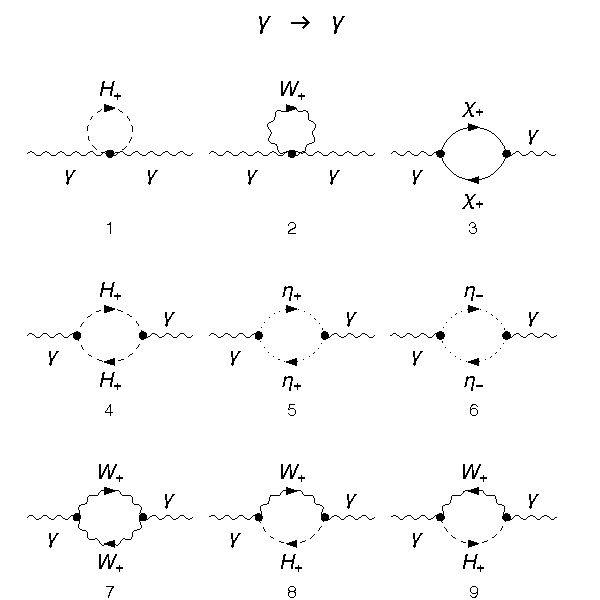
\includegraphics[width=0.6\textwidth]{diagrams_V[1]_1.pdf}
\caption{The one-loop corrections to the photon propagator.}\label{fig:gammagamma}
\end{figure}

From Ibe et al. we have
\begin{align}
\Pi_{\gamma \gamma}^{(V, h)}(p^2) =
-\frac{3 \hat{e}^2}{4\pi^2}
\left[ \tilde{B}_{22}(p^2, \hat{m}_W^2, \hat{m}_W^2) + \frac{p^2}{18} \right]
-\frac{\hat{e}^2 p^2}{4\pi^2} B_0(p^2, \hat{m}_W^2, \hat{m}_W^2) \label{eqn:gammagamma}
\end{align}
where this includes all contributions from the 9 diagrams in Figure \ref{fig:gammagamma}.  We find the self energy contribution from \mb i a fully reduced scheme is
\begin{align}
\Pi_{\gamma \gamma}^{(V, h)}(p^2) = \frac{\alpha}{32\pi^2} \left( \left(4m_W^2-6(2m_W^2+p^2)\right)B_0(m_W^2,m_W^2)+8 A_0(m_W^2)-8m_W^2\right)
\end{align}
which is equivalent to (\ref{eqn:gammagamma}) after using the tensor integral reduction relationships given in section \ref{app:reduction}.

\begin{figure}[b!]
\center
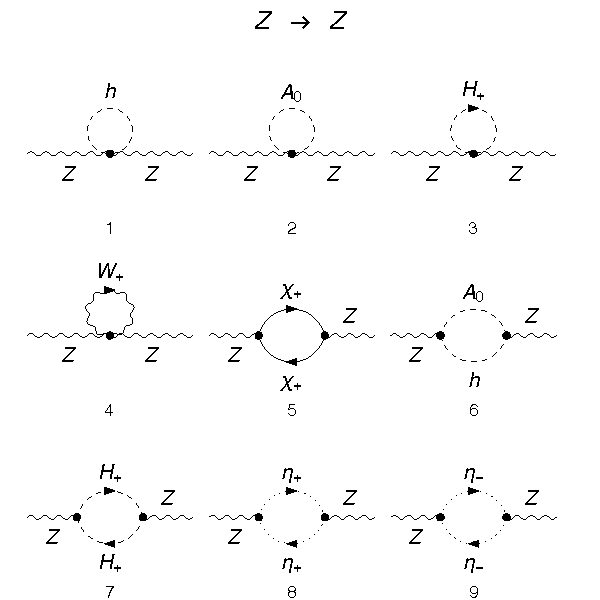
\includegraphics[width=0.5\textwidth]{diagrams_V[2]_1_1.pdf}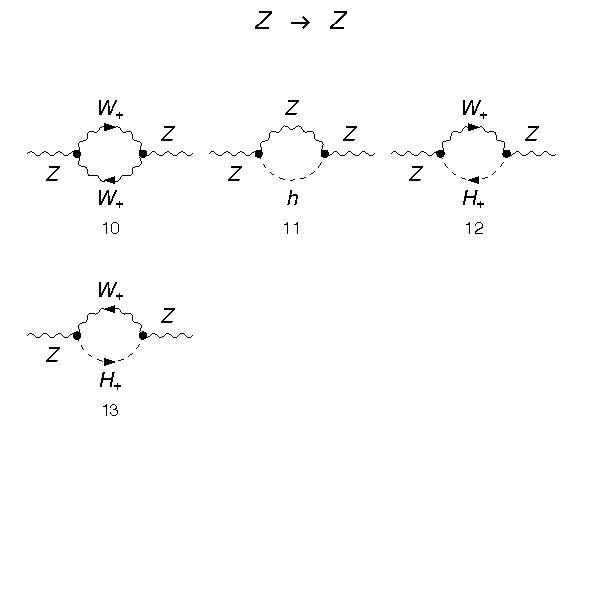
\includegraphics[width=0.5\textwidth]{diagrams_V[2]_1_2.pdf}
\caption{The one-loop corrections to the Z boson propagator.}\label{fig:ZZ}
\end{figure}

\subsubsection{Z boson self energy}

The Z boson self energy as given by Ibe et al. is
{
\begin{eqnarray}
\Pi_{ZZ}^{(V,h)}(p^2) &=& 
-\frac{ \hat{g}^2 (12\hat{c}_W^4 - 4\hat{c}_W^2 + 1) }{16\pi^2 \hat{c}_W^2}
\tilde B_{22}(p^2, \hat{m}_W^2, \hat{m}_W^2) 
-\frac{ \hat{g}^2 \hat{c}_W^2 p^2 }{24\pi^2} \nonumber \\
&& -\frac{2\hat{g}^2}{16\pi^2}(2\hat{c}_W^2 p^2 + 2\hat{m}_W^2 - \hat{m}_Z^2)
B_0(p^2, \hat{m}_W^2, \hat{m}_W^2) \nonumber \\
&& -\frac{ \hat{g}^2 }{16\pi^2 \hat{c}_W^2}
[\tilde B_{22}(p^2, \hat{m}_Z^2, \hat{m}_h^2)\label{eqn:ZZ}
-\hat{m}_Z^2 B_0(p^2, \hat{m}_Z^2, \hat{m}_h^2) ]
\end{eqnarray}
}
the result from \mb is
{
\begin{eqnarray}
\Pi_{ZZ}^{(V,h)}(p^2) &=& 
-\frac{ \hat{g}^2} {576 c_W^4 p^2 \pi^2}\left\{
2 p^2 \left[-3 m_H^2 (-1 + s_W^2) + 2 p^2 (1 - 3 s_W^2 + 2 s_W^4) \right. \right.\nonumber\\
&& \left.+ 3 m_W^2 (19 - 58 s_W^2 + 64 s_W^4 - 24 s_W^6)\right] \nonumber\\
&&- 3 (m_W^2 + m_H^2 (-1 + s_W^2) - 2 p^2 (-1 + s_W^2)) A0\left(m_H^2\right)  \nonumber\\
 &&  + 12 p^2 (-9 + 29 s_W^2 - 32 s_W^4 + 12 s_W^6) A_0\left(m_W^2\right)  \nonumber\\
   && +3 ((m_W^2 + m_H^2 (-1 + s_W^2) + 2 p^2 (-1 + s_W^2)) A0\left(m_Z^2\right)  \nonumber\\
   &&+ \left[-m_W^2 (m_Z^2 + 10 p^2) + m_H^4 (-1 + s_W^2)\right.  \nonumber\\
   && \left. +     p^4 (-1 + s_W^2) + 2 m_H^2 (m_W^2 - p^2 (-1 + s_W^2))\right] B_0\left(p^2, m_H^2, m_Z^2\right)  \nonumber\\
&&   -    p^2 (-1 + s_W^2) \left[4 m_W^2 (15 - 32 s_W^2 + 12 s_W^4)\right.  \nonumber\\
&&  \left.      \left. +  p^2 (39 - 76 s_W^2 + 36 s_W^4)\right] B_0\left(p^2, m_W^2, m_W^2\right)))\right\}
\end{eqnarray}
}
which is equivalent to (\ref{eqn:ZZ}) after using the appropriate reduction relationships.




\begin{figure}[h!]
\center
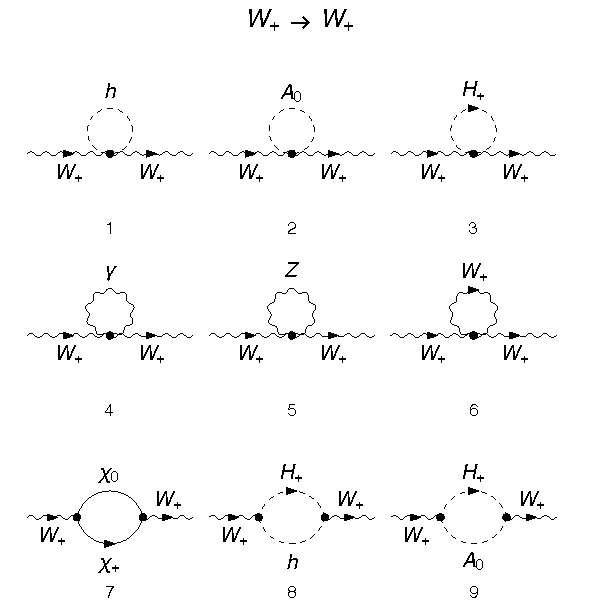
\includegraphics[width=0.5\textwidth]{diagrams_V[3]_1_1.pdf}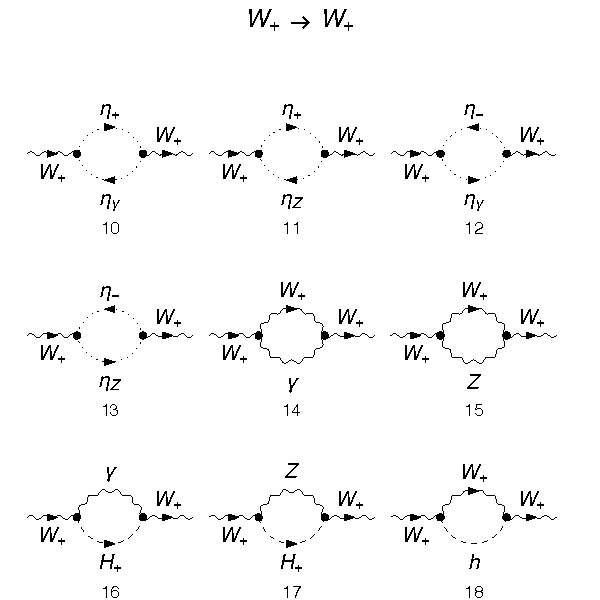
\includegraphics[width=0.5\textwidth]{diagrams_V[3]_1_2.pdf}
\caption{The one-loop corrections to the W boson propagator.}\label{fig:WW}
\end{figure}

\subsubsection{W boson self energy}
The W boson self energy is given by Ibe et al. to be
{\small
\begin{eqnarray}
\Pi_{WW}^{(V, h)}(p^2) &=&
-\frac{8\hat{e}^2}{16\pi^2} \tilde B_{22}(p^2, 0, \hat{m}_W^2)
-\frac{\hat{e}^2 p^2}{24\pi^2}
-\frac{4\hat{e}^2 p^2}{16\pi^2} B_0(p^2, 0, \hat{m}_W^2) \nonumber \\
&& -\frac{\hat{g}^2}{16\pi^2}(1 + 8\hat{c}_W^2)
\tilde{B}_{22}(p^2, \hat{m}_W^2, \hat{m}_Z^2)
-\frac{\hat{g}^2 \hat{c}_W^2 p^2}{24\pi^2} \nonumber \\
&& -\frac{\hat g^2}{16\pi^2}( 4 \hat c_W^2 p^2 + 3 \hat m_W^2 - \hat m_Z^2) B_0( p^2, \hat m_W^2, \hat m_Z^2) \nonumber\\
&& -\frac{\hat{g}^2}{16\pi^2}
[ \tilde{B}_{22}(p^2, \hat{m}_W^2, \hat{m}_h^2)
-\hat{m}_W^2 B_0(p^2, \hat{m}_W^2, \hat{m}_h^2) ]\ .\label{eqn:WW}
\end{eqnarray}
}

We compute the self energy using \mb and find a consistent result if $m_{\gamma}=0$.  
{
\begin{eqnarray}
\Pi_{WW}^{(V,h)}(p^2) &=& 
-\frac{ \hat{g}^2} {576 c_W^4 p^2 \pi^2}\left\{ -6 m_H^2 p^2 - 4 p^4 \right.+  24 (m_{\gamma}^2 - m_W^2 - 2 p^2) s_W^2 (-1 + s_W^2) A_0(m_{\gamma}^2) -  \nonumber\\
&&   3 m_H^2 A_0(m_H^2) + 6 p^2 A_0(m_H^2) + 3 m_H^2 A_0(m_W^2) + 60 p^2 A_0(m_W^2) + 54 p^2 A_0(m_Z^2)\nonumber \\
&&   + 3 m_H^4 B_0(p^2, m_H^2, m_W^2) -6 m_H^2 p^2 B_0(p^2, m_H^2, m_W^2) + 3 p^4 B_0(p^2, m_H^2, m_W^2) + \nonumber\\
&&   3 m_W^4 (B_0(p^2, m_H^2, m_W^2) - B_0(p^2, m_W^2, m_Z^2))\nonumber \\
&&   + 3 m_W^2 m_Z^2 B_0(p^2, m_W^2, m_Z^2) - 117 p^4 B_0(p^2, m_W^2, m_Z^2) \nonumber\\
&&   + 24 m_W^4 s_W^4 (-B_0(p^2, m_{\gamma}^2, m_W^2) + B_0(p^2, m_W^2, m_Z^2))\nonumber \\
&&   + 24 m_W^2 s_W^4 (A_0(m_Z^2) + 2 (m_{\gamma}^2 + p^2) B_0(p^2, m_{\gamma}^2, m_W^2) - 2 p^2 B_0(p^2, m_W^2, m_Z^2))\nonumber \\
&&   - 12 s_W^4 \left[    2 m_{\gamma}^2 A_0(m_W^2) -  4 p^2 (m_{\gamma}^2 + A_0(m_Z^2)) \right.\nonumber \\
&& \left. + (2 m_{\gamma}^4 - 7 m_{\gamma}^2 p^2 - 10 p^4) B_0(p^2,m_{\gamma}^2, m_W^2) + 10 p^4 B_0(p^2, m_W^2, m_Z^2]\right] \nonumber\\
&&  + m_W^4 s_W^2 (24 B_0(p^2, m_{\gamma}^2, m_W^2) - 3 (B_0(p^2, m_H^2, m_W^2) + B_0(p^2, m_W^2, m_Z^2))) \nonumber\\
&&   +  s_W^2 \left[-48 m_{\gamma}^2 p^2 + 6 m_H^2 p^2 + 4 p^4 +  3 (m_H^2 - 2 p^2) A_0(m_H^2)
\right.\nonumber\\
&&   +  3 (8 m_{\gamma}^2 - m_H^2 - 20 p^2) A_0(m_W^2) +   24 m_{\gamma}^4 B_0(p^2, m_{\gamma}^2, m_W^2) - 3 m_H^4 B_0(p^2, m_H^2, m_W^2) - \nonumber\\
&&    3 p^2 (34 A_0(m_Z^2) + 4 (7 m_{\gamma}^2 + 10 p^2) B_0(p^2, m_{\gamma}^2, m_W^2) + (-2 m_H^2 + p^2) B_0(p^2, m_H^2, m_W^2) \nonumber\\
&& \left.- 79 p^2 B_0(p^2, m_W^2, m_Z^2))\right]    \nonumber\\
&& +  3 m_W^2 (A_0(m_H^2) - A_0(m_W^2) -  2 ((m_H^2 - 5 p^2) B_0(p^2, m_H^2, m_W^2)\nonumber\\
&&       + p^2 (19 + 30 B_0(p^2, m_W^2, m_Z^2))))\nonumber \\
&&     - 3 m_W^2 s_W^2 \left[A_0(m_H^2) - 2 A_0(m_W^2) + 9 A_0(m_Z^2) + 2 (8 (m_{\gamma}^2 + p^2) B_0(p^2, m_{\gamma}^2, m_W^2) \right.\nonumber\\
&& \left. \left .- (m_H^2 - 5 p^2) B_0(p^2, m_H^2, m_W^2) - p^2 (18 + 43 B_0(p^2, m_W^2, m_Z^2)))\right] \right\}\label{eqn:mb_WW}
\end{eqnarray}
}
which after performing the reduction on (\ref{eqn:WW}) but before setting $m_{\gamma}=0$ in (\ref{eqn:mb_WW}) we find an additional term
\begin{align}
\Pi_{WW}^{\text{\mb}}  - \Pi_{WW}^{\text{Ibe}}  =\frac{g_2^2 m_{\gamma}^2 s_W^2 B_0(p^2,m_{\gamma}^2,m_W^2)}{16 \pi^2}
\end{align}
which is zero for $m_{\gamma}=0$.  This is the only difference between our working and that of Ibe et al. where they have clearly just set $m_{\gamma}=0$ in the published result.



\subsection{1-loop counter-terms}

We determine the one-loop counter-term couplings using the inbuilt Mass Builder feature.  After all diagrams have been computed, Mass Builder collects all amplitudes together and extracts the coefficient of $1/\epsilon$ and simplifies this to give the one-loop counter term coupling\footnote{This is straightforward as the problem is reduced to a linear algebraic equation, at the two-loop level the problem involves solving a well choosen set of simultaneous equations so is currently not supported.}.  It also prints out the coefficients of $1/\epsilon^2$ and $1/\epsilon^3$ as a check that higher order divergences do not exist in the one-loop amplitude.  With this method we determine the following counter-terms
\begin{eqnarray}
\delta_{Z_{WW}} &=&- \frac{g_2^2}{16 \pi^2}\left(-\frac{11}{6}\right),\\
\delta_{m^2_{WW}}&=&- \frac{g_2^2}{16 \pi^2} \left( m^2_Z(-1+2s_W^2)     -m_{\gamma}^2s_W^2\right),\\
\delta_{Z_{\gamma\gamma}} &=&-\frac{g_2^2s_W^2}{16 \pi^2}\left(-\frac{5}{3}\right) = \frac{\hat{e}^2}{16\pi^2}\left(-\frac{5}{3}\right) , \\
%%%%%
\delta_{m^2_{\gamma\gamma}} &=& 0\, ,\\
\delta_{Z_{ZZ}} &=&-\frac{g_2^2}{16 \pi^2 c_W^2} \left(-\frac{11}{6}+\frac{11}{3}s_W^2-\frac{5}{3}s_W^4  \right),\\
\delta_{m^2_{ZZ}} &=& -\frac{g_2^2m_Z^2}{16 \pi^2c_W^2} \left(-1+6s_W^2-4s_W^4  \right),\\
\delta_{m^2_{Z\gamma}} &=& -\frac{g_2^2s_W}{16 \pi^2c_W} \left( m_Z^2(2-2s_W^2)  \right),\\
\delta_{Z_{Z\gamma}} &=& -\frac{g_2^2s_W}{16 \pi^2c_W} \left( \frac{11}{6}-\frac{5s_W^2}{3}  \right)
\end{eqnarray}

These match those of Ibe et al. (if we neglect the terms which obviously come from the SM fermionic and leptonic interactions -- which our model does not contain) for the case of $m_{\gamma}=0$.  As there is mixing between the Z boson and the photon we also computed a counter-term coupling for the two point propagator $Z\rightarrow\gamma$.  This mixing calculation is fully supported in \mb by using the additional \lstinline{-q <particle>} option.

The one-loop counter-term couplings for the fermionic triplet are computed in the same way to give
\begin{eqnarray}
\delta_{Z_{\chi^0\chi^0}} &=&-\frac{g_2^2}{8 \pi^2}\\
\delta_{M_{\chi^0\chi^0}} &=&-\frac{g_2^2 M}{2 \pi^2}
\end{eqnarray}
which agree with that of Ibe et al.


\subsubsection{Gauge interaction of the triplet}

Finally we need the counter-term for the interaction between the triplet and the gauge sector.  This is given by Ibe et al. in the following direct quote:\\

\textcolor{blue}{
The neutral and charged winos have the SU(2)$_L$ gauge interaction which is described by the term, ${\cal L}_{\rm int} = i\epsilon_{abc}(\hat{g} + \delta_{\tilde{\chi} \tilde{\chi} W}) \tilde{\chi}^{a \dagger} \slashed{W}^b \tilde{\chi}^c$, and the counter-term is given by
\begin{eqnarray}
\delta_{\tilde{\chi} \tilde{\chi} W} = \frac{\hat{g}^3}{4\pi^2} \Delta\ .
\end{eqnarray}
}

The notation that has been used here is not clear.  From an understanding of the Lagrangian, we know that there are more interactions than just those between the electroweak triplet (here referred to as a wino) and the W boson, so we must infer that $ \slashed{W}^a = \{W^+,W^-,W^3\}$ where $W_{\mu}^3 = (s_W A_{\mu}+c_W Z_{\mu})$ (see \cite{Ostdiek2015} for an example of this notation).  This would give us the following renormalised Lagrangian
\begin{align}
\begin{split}
\mathcal{L}=
&(g+\delta_{\tilde{\chi} \tilde{\chi} W})\left(\overline{\mychi^+}\gamma_{\mu}\mychi^+\right)\left(s_WA_{\mu}+c_WZ_{\mu}\right)\\
&+(g+\delta_{\tilde{\chi} \tilde{\chi} W})\left(\overline{\mychi^+}\gamma_{\mu}\mychi^0 \right)W_{\mu}^++\text{h.c.}\\
&=g\left(\overline{\mychi^+}\gamma_{\mu}\mychi^+\right)\left(s_wA_{\mu}+c_wZ_{\mu}\right)+\left[g\left(\overline{\mychi^+}\gamma_{\mu}\mychi^0 \right)W_{\mu}^++\text{h.c.}\right]\\
&+s_W\delta_{\tilde{\chi} \tilde{\chi} W}\left(\overline{\mychi^+}\gamma_{\mu}\mychi^+\right)A_{\mu}+c_W\delta_{\tilde{\chi} \tilde{\chi} W}\left(\overline{\mychi^+}\gamma_{\mu}\mychi^+\right)Z_{\mu}\\
&+\left[\delta_{\tilde{\chi} \tilde{\chi} W}\left(\overline{\mychi^+}\gamma_{\mu}\mychi^0 \right)W_{\mu}^++\text{h.c.}\right]\\
\end{split}
\end{align}

so the resultant counter-terms we need to add into the calculation are $\delta_{\tilde{\chi} \tilde{\chi} W}$, $s_W\,\delta_{\tilde{\chi} \tilde{\chi} W}$ and $c_W\,\delta_{\tilde{\chi} \tilde{\chi} W}$ for the $W\chi\chi^{\dagger}$, $A\chi\chi$ and $Z\chi\chi$ vertices respectively.
\newpage
\subsection{2-loop self energy}

We are finally ready to compute the two-loop self energy for the electroweak triplet.  For the neutral (charged) component there are 48 (75) two-loop diagrams and eight (10) counter-term diagrams of two-loop order.\\

To compute the pole mass correctly, and thus the mass splitting, we also need to evaluate the derivatives of the one-loop self energies.  This is not required if we are to compute the pole mass via the iterative method, but we will leave that until a later section.  The derivates of the one loop self energies were computed by hand and are provided with \mb in the \lstinline{supplements} \lstinline{namespace} defined in the file \lstinline{src/supplements.cpp}.  The \lstinline{triplet} \lstinline{cmake} target creates an executable that will retrieve both the two-loop amplitudes and the derivatives of the one-loop self energies to produce the full two-loop mass splitting.\\

Figures \ref{fig:chi1chi1_2}, \ref{fig:chi1chi1_1}, \ref{fig:chi0chi0} and \ref{fig:chi_ct2} give the diagrams of two-loop order.
\begin{figure}[h!]
\center
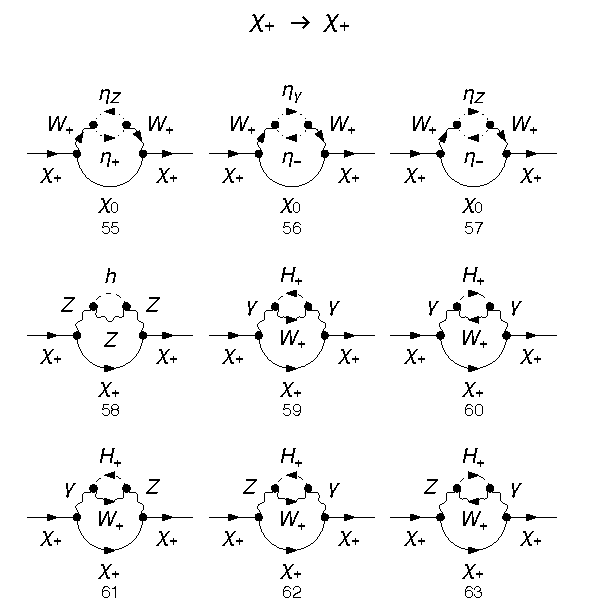
\includegraphics[width=0.5\textwidth]{diagrams_F[1]_2_7.pdf}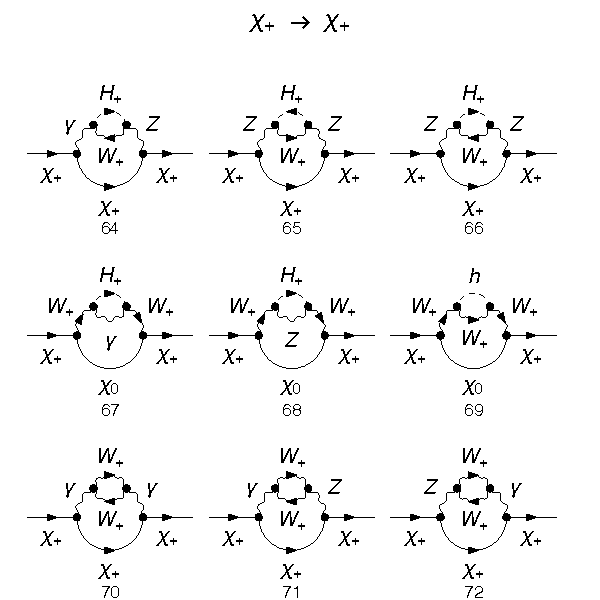
\includegraphics[width=0.5\textwidth]{diagrams_F[1]_2_8.pdf}
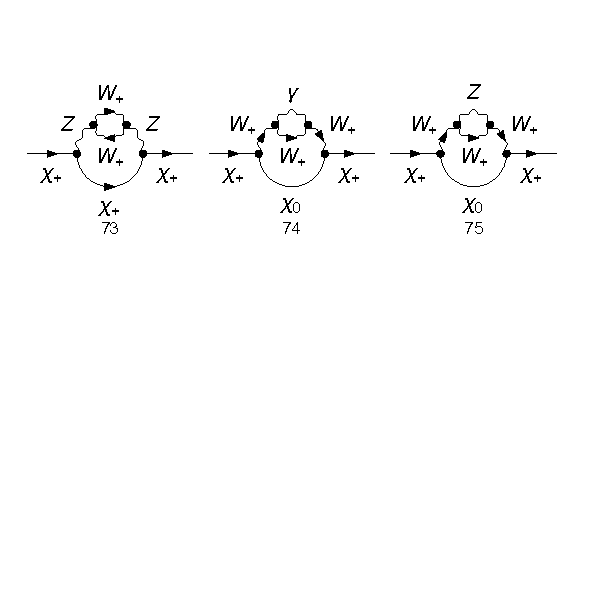
\includegraphics[width=0.5\textwidth]{diagrams_F[1]_2_9.pdf}
\caption{The two-loop corrections to the $\chi^+$ propagator.}\label{fig:chi1chi1_2}
\end{figure}

\begin{figure}[h!]
\center
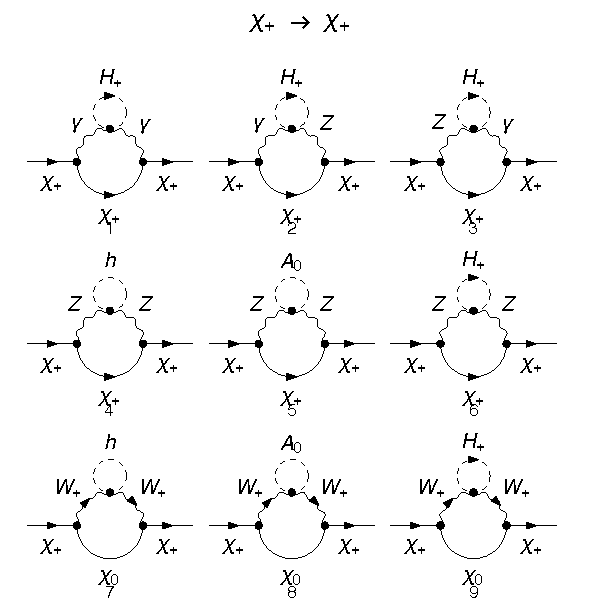
\includegraphics[width=0.5\textwidth]{diagrams_F[1]_2_1.pdf}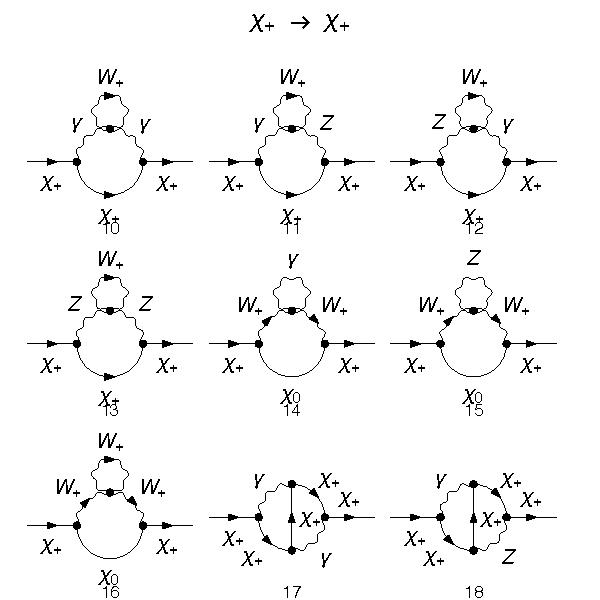
\includegraphics[width=0.5\textwidth]{diagrams_F[1]_2_2.pdf}
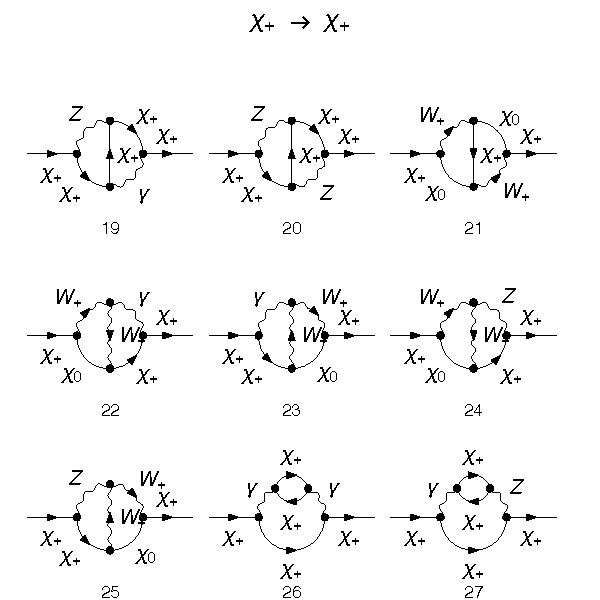
\includegraphics[width=0.5\textwidth]{diagrams_F[1]_2_3.pdf}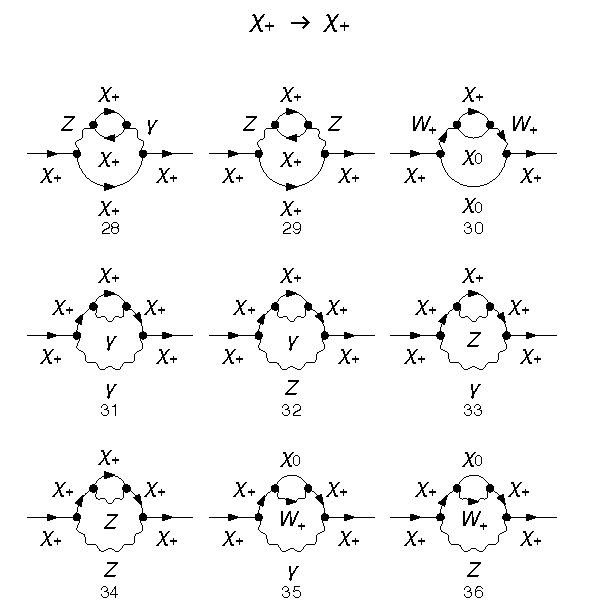
\includegraphics[width=0.5\textwidth]{diagrams_F[1]_2_4.pdf}
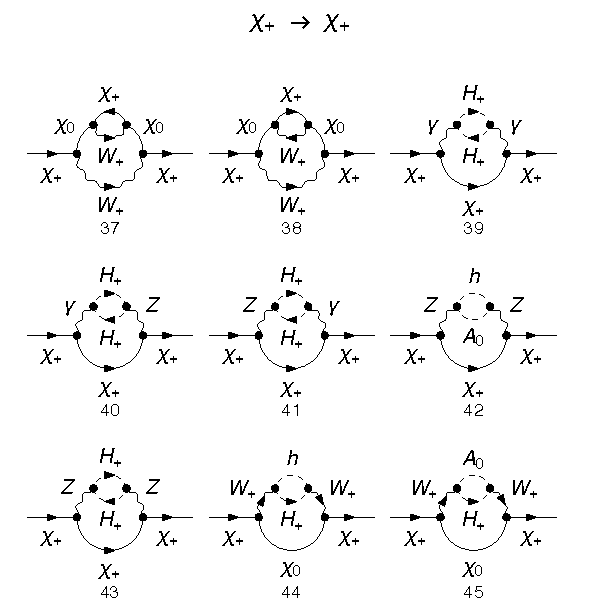
\includegraphics[width=0.5\textwidth]{diagrams_F[1]_2_5.pdf}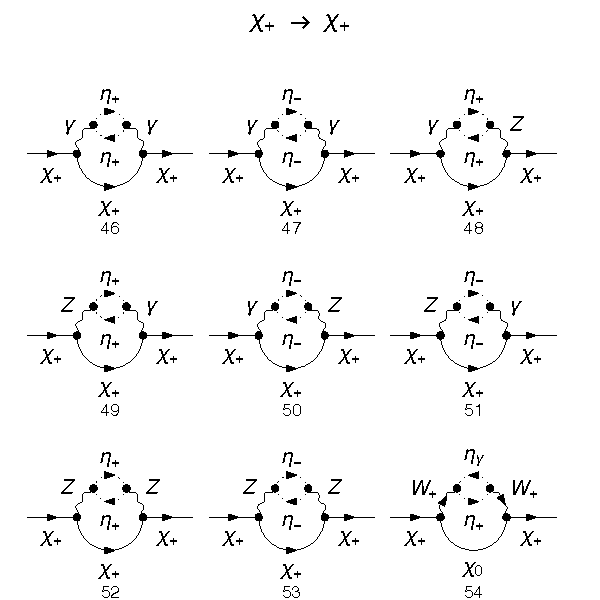
\includegraphics[width=0.5\textwidth]{diagrams_F[1]_2_6.pdf}
\caption{The two-loop corrections to the $\chi^+$ propagator.}\label{fig:chi1chi1_1}
\end{figure}



\begin{figure}[h!]
\center
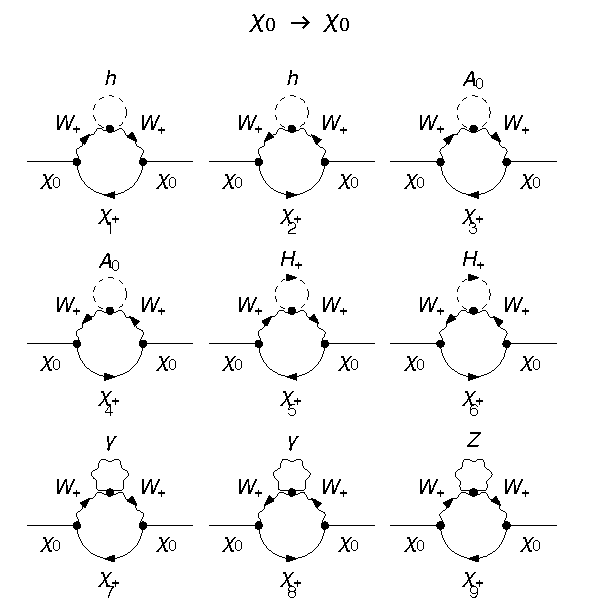
\includegraphics[width=0.5\textwidth]{diagrams_F[2]_2_1.pdf}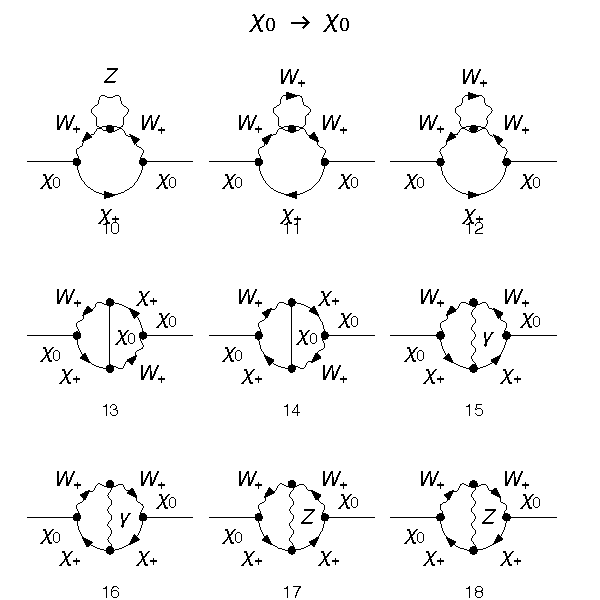
\includegraphics[width=0.5\textwidth]{diagrams_F[2]_2_2.pdf}
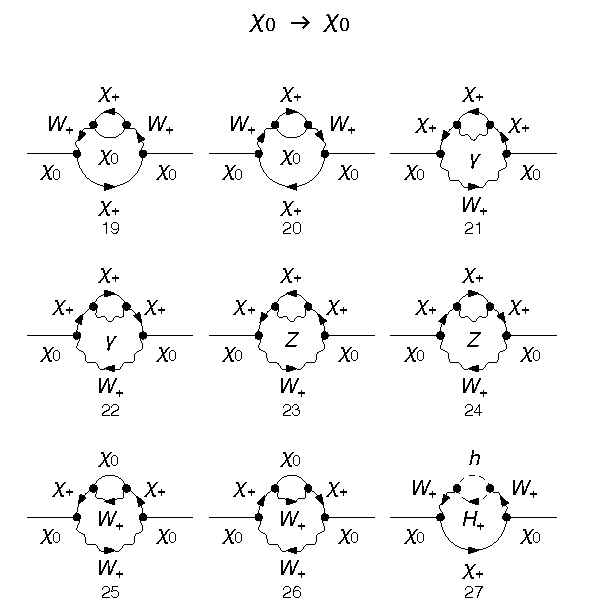
\includegraphics[width=0.5\textwidth]{diagrams_F[2]_2_3.pdf}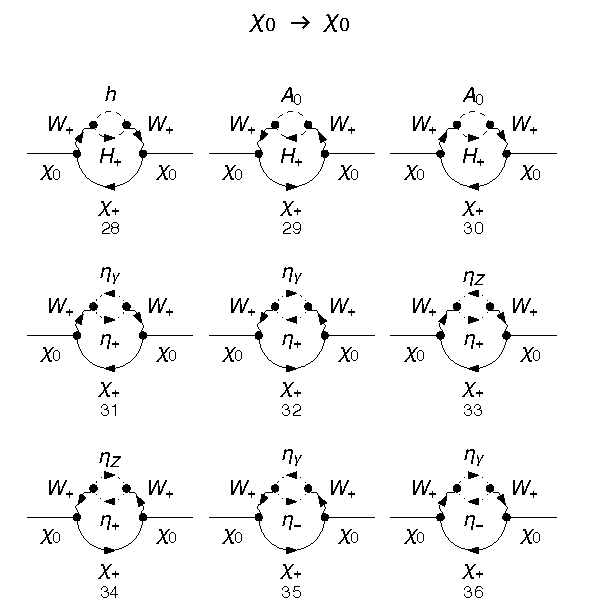
\includegraphics[width=0.5\textwidth]{diagrams_F[2]_2_4.pdf}
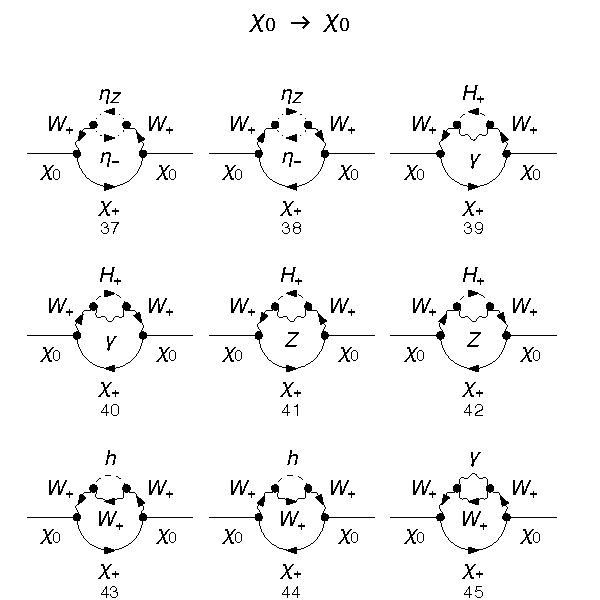
\includegraphics[width=0.5\textwidth]{diagrams_F[2]_2_5.pdf}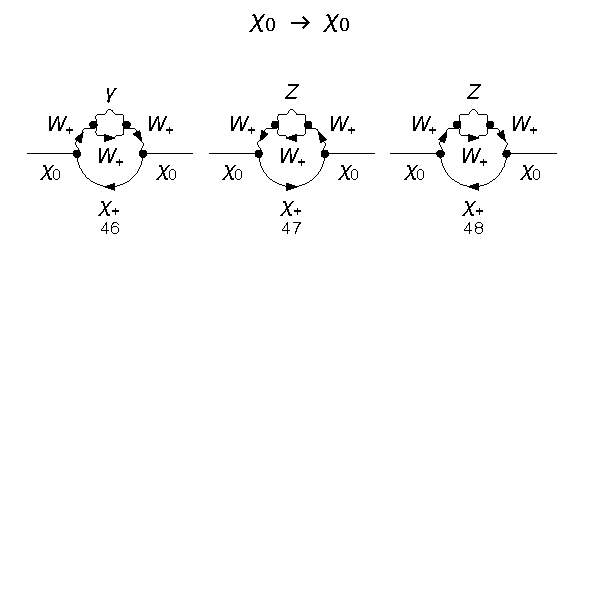
\includegraphics[width=0.5\textwidth]{diagrams_F[2]_2_6.pdf}
\caption{The two-loop corrections to the $\chi^0$ propagator.}\label{fig:chi0chi0}
\end{figure}



\begin{figure}[h!]
\center
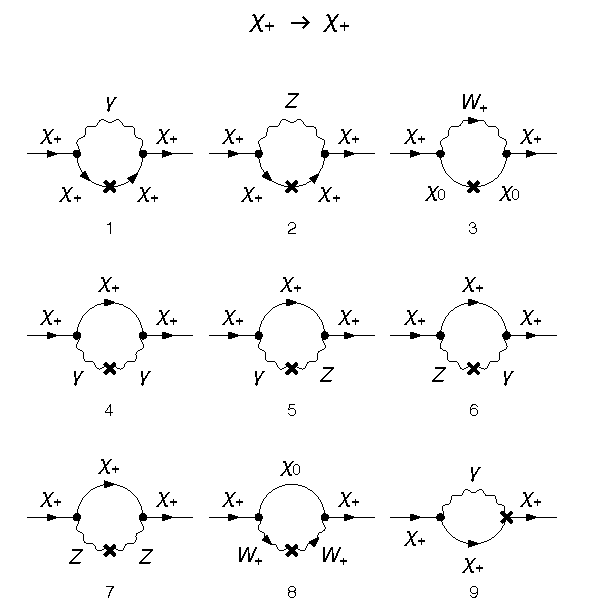
\includegraphics[width=0.5\textwidth]{diagrams_F[1]_2c_1.pdf}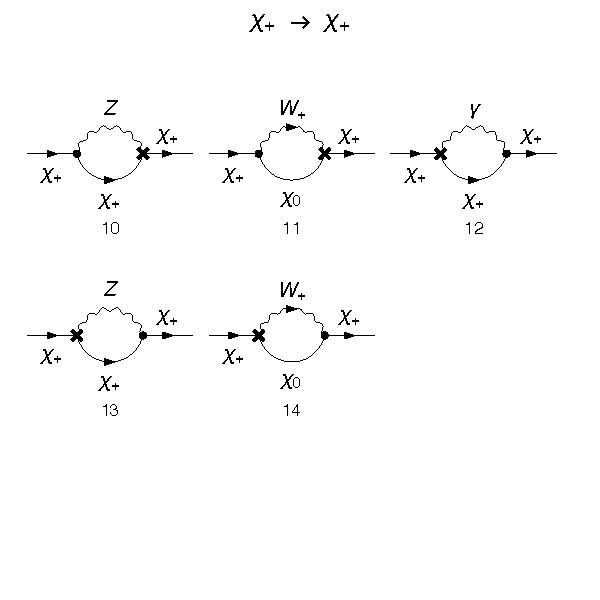
\includegraphics[width=0.5\textwidth]{diagrams_F[1]_2c_2.pdf}
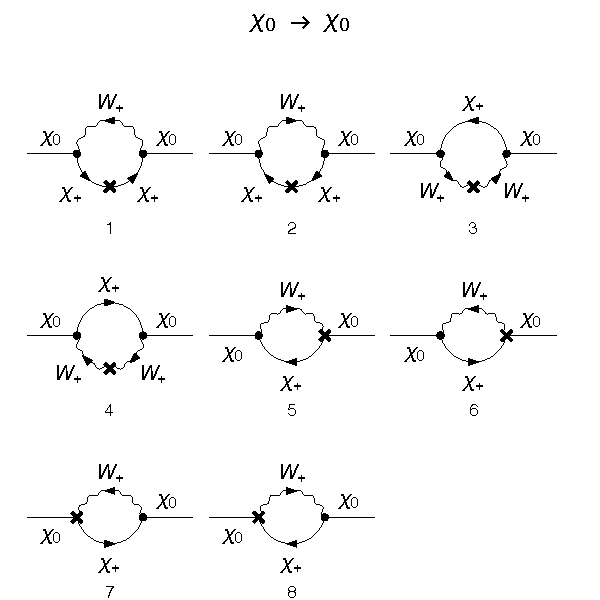
\includegraphics[width=0.5\textwidth]{diagrams_F[2]_2c.pdf}
\caption{The two-loop order counter-terms corrections to the $\chi^+$ and $\chi^0$ propagators.}\label{fig:chi_ct2}
\end{figure}

\clearpage

\subsubsection{IR divergences}

We expect there to be IR divergence arising from a specific set of diagrams, as described by Ibe et al. in the following:\\

\textcolor{blue}{
For the charged wino, the amplitude in Figure (reference) in which a photon is circulating
in the outer loop and the one in [the counter-term diagram] Figure (reference) with the photon loop behave as
\begin{eqnarray}
\Sigma_{K,M}^{(2)}(p^2=\hat{M}_2^2) \sim
\int \frac{d^4 k}{(2\pi)^4} \frac{1}{(k\cdot p)^2} \frac{1}{k^2} \ ,
\end{eqnarray}
and hence, they are IR divergent.
In addition, the derivatives, $\dot{\Sigma}_{K,M}^{(1)} |_{p^2=\hat{M}_2^2}$, 
are also IR divergent due to the diagram including a photon propagator. 
}\\

In our approach we wish to set a finite mass for the photon, as this still gives the same phenomenology for the mass splittings at the one-loop level.  Therefore any interesting effects at the two-loop level should be able to be studied with a small but finite photon mass.  The cancellation between IR divergences mentioned above should also occur numerically if we set a small photon mass, resulting in a still reasonable total amplitude.\\

However, we find that there are significantly more diagrams which are ill-defined in the limit of $m_{\gamma}\rightarrow 0$.  We have two options when computing these.  First, we can either set $m_{\gamma}=0$ from the outset, then we will end up with an amplitude proportional to $(p^2-M^2)^{-1}$, which is ill-defined for the important case of $p^2=M^2$ (either in the implicit or explicit calculation of the pole mass, the amplitudes must be finite here).  The second option is to leave a finite $m_{\gamma}$ throughout the calculation and subsequent basis integral reduction, and substitute $m_{\gamma}\rightarrow 0$ at the end.  This results in an amplitude proportional to $m_{\gamma}^{-2}$ or in a basis integral which is not defined at $m_{\gamma}=0$, so again this is ill-defined.\\

One possibility is that our diagram by diagram approach is flawed because of missing cancellations between diagrams.  To investigate this we compute the diagrams with a finite $m_{\gamma}$ throughout and then attempt to evaluate the result with $m_{\gamma}=0$.  The IR divergence is not always evident from a $m_{\gamma}^{-2}$ factor as it may be that one of the basis integrals is ill-defined, so we check that a diagram is finite by numerical evaluation.  We then compose a list of diagrams which are undefined (in this case all returning an \lstinline{inf} result) and sum these together.  If there is any important cancellation that would solve the problem, it would occur between these ill-defined diagrams, and not from any other finite diagram.  So we only have a handful of amplitudes to sum together, which is an achievable yet still cumbersome task for an analytical simplifier.  We find that the resultant sum still containts integrals which are ill-defined at $m_{\gamma}=0$, such as $T(m_{\gamma},M,m_W)$.\\

So we find that for the neutral component of the triplet, every diagram which includes a photon propagator, in any leg, is IR divergent, and the sum of these is also IR divergent.


\subsubsection{Numerical results}

The most powerful feature of \mb is to automatically generate an interface to \tsil for the resultant self energy amplitudes.  This provides a fast and more importantly free-from-errors method of obtaining a numerical result for the self energies at one and two-loop order.\\

The input parameters and resultant self energies and pole masses are given in Table \ref{table:input_params}.

\begin{table}[h!]
\caption{The parameter values used for the electroweak triplet self energy calculations.  Where a derived quantity is used this is passed directly to \mb in the analytic form.}\label{table:input_params}
\centering
\vspace{0.5cm}
\begin{tabular}{l l}
\hline
Parameter & Value\\
\hline
$m_W$ & $80.385$ GeV \\
$m_Z$ & $91.1876$ GeV \\
$m_H$ & 125.6 GeV\\
$M$ & 100 GeV\\
$m_{\gamma}$ & 0 \\
$v$ & 246 GeV \\
$Q$ & 100 GeV \\
$c_W^2$ & $m^2_W/m^2_Z$ \\
$s_W^2$ & $1-c^2_W$ \\
$g_2$ & $2m_W/v$\\
$g_1$ & $g_2 s_W/c_W$\\
\hline\end{tabular}
\hspace{3cm}
\begin{tabular}{l l}
\hline
Field & 1-loop self energy (GeV)\\
\hline
$W$ & $-$ \\
$Z$ & $-$  \\
$\gamma$ & $-$ \\
$\chi^+$ & $-$ \\
$\chi^0$ & $-$ \\
&\\
\hline
Field & 2-loop self energy (GeV)\\
\hline
$\chi^+$ & $-$ \\
$\chi^0$ & $-$ \\
&\\
\hline
Field & Physical mass (GeV)\\
\hline
$W$ & $-$ \\
$Z$ & $-$  \\
$\gamma$ & $-$\\
\hline\end{tabular}
\end{table}


\newpage
\section{Appendix -- Definitions}

We will make use of tools and literature sources which use slightly different definitions for the same mathematical objects.  In this section we make it clear what these differences are and how these differences alter the important relationships between these objects.


In the following I use bold-face for the divergent integrals and normal type for the finite pieces, as defined in the TSIL manual.  I use $\tt{TAI}$ to refer to TARCER notation and $A$ for TSIL notation as there is a different normalisation between such integrals.  We define $\kappa = 1/16\pi^2$.

We begin with $B_0$ and $B_1$.  These are defined by Ibe at al. as
\begin{eqnarray}
B_0(p^2, m_1^2, m_2^2) &=& \Delta
- \int_0^1 dx ~\log \frac{ (1-x)m_1^2 + x m_2^2 - x(1-x)p^2 -i\epsilon }{Q^2}\ , \\
B_1(p^2, m_1^2, m_2^2) &=& -\frac{\Delta}{2}
+ \int_0^1 dx ~x\log \frac{ (1-x)m_1^2 + x m_2^2 - x(1-x)p^2 -i\epsilon }{Q^2}\ , \\
B_{21}(p^2, m_1^2, m_2^2) &=& \frac{\Delta}{3}
- \int_0^1 dx ~x^2\log \frac{ (1-x)m_1^2 + x m_2^2 - x(1-x)p^2 -i\epsilon }{Q^2}\ ,
\end{eqnarray}

while BMPZ defines these as
\begin{eqnarray}
A_0(m) &=& 16\pi^2Q^{4-n}\int{d^nq\over i\,(2\pi)^n}{1\over
q^2-m^2+i\varepsilon}\\
B_0(p, m_1, m_2) &=&
16\pi^2Q^{4-n}\int{d^nq\over i\,(2\pi)^n}
{1\over\biggl[q^2-m^2_1+i\varepsilon\biggr]\biggl[
(q-p)^2-m_2^2+i\varepsilon\biggr]}
\label{B0 def}  \\
p_\mu B_1(p, m_1,m_2) &=& 16\pi^2Q^{4-n}\int
{d^nq\over i\,(2\pi)^n}{q_\mu\over\biggl[q^2-m^2_1+i\varepsilon\biggr]
\biggl[(q-p)^2-m_2^2+i\varepsilon\biggr]}\label{B1 def} \\ p_\mu p_\nu
B_{21}(p,m_1,m_2) &+& g_{\mu\nu}B_{22}(p,m_1,m_2)
\label{B22 def}\\
 &=& 16\pi^2\,Q^{4-n}\,\int{d^nq\over i\,(2\pi)^n} {q_\mu
q_\nu\over\biggl[q^2-m^2_1+i\varepsilon\biggr]\biggl[
(q-p)^2-m_2^2+i\varepsilon\biggr]}\ , \nonumber
\end{eqnarray}
where we deal with $B_{22}$ later.  

The above definitions are not equivalent, first we need to set $\Delta = 2/(4-D)-\gamma_E+\log(4\pi)$ and $n=D$.  However, there is an important sign difference from the way the denominator is written.  BMPZ use $(p-k)$ while other sources, including Ibe et al. use $(p+k)$.  Therefore when doing the Feynman integration and introducing the step, we end up shifting the integration measure, $k$, by either $k+px$ or $k-px$.  This difference introduces a sign difference in the integrated form of $B_1$.  (need to check the validity of the relationship given in B.9 in BMPZ for the case of $(k+p)$.  \textcolor{red}{Therefore when we compare with the results stated in Ibe et al. we must be careful with the sign of the $B_1$ integral and make sure to introduce a negative.}
TSIL defines
\begin{eqnarray}
{\bf A}(x) &=&  
C \int d^d k \frac{1}{[k^2 +x]}  %,
\label{defineboldA}
\\
{\bf B}(x,y) &=&
C \int d^d k   \frac{1}{[k^2 +x] [(k-p)^2 +y]} .
\label{defineboldB}
\end{eqnarray}
where
\begin{equation}
C = (16 \pi^2) \frac{\mu^{2\epsilon}}{(2 \pi)^d}
  = (2 \pi \mu)^{2 \epsilon}/\pi^2 .
\end{equation}
and TARCER uses

\begin{eqnarray}
{\bf A}(x) &=& i \cTarasov \mbox{{\tt TAI$[$d,s,$\{\{1,\sqrt{x}\}\}]$}},
\\
{\bf B}(x,y) &=& -i \cTarasov \mbox{{\tt TBI$[$d,s,$\{%
\{1,\sqrt{x}\},\{1,\sqrt{y}\}\}]$}} 
\end{eqnarray}
where 
$
\cTarasov = (4 \pi \mu^2)^{2-d/2}.
$
So we make the identification that $n=D=4-2\epsilon$ and achieve equivalent pre-factors.  There is an important sign difference attached to the $m^2=x$ quantity between the different definitions of $A_0$ and $B_0$.  The effects the form of the finite plus divergent expansion of the basis integrals.  From the TSIL manual we have
\begin{eqnarray}
{\bf A}(x) &=& -x/\epsilon + A(x) + \epsilon A_\epsilon(x) + 
{\cal O}(\epsilon^2) 
\\
{\bf B}(x,y) &=& 1/\epsilon + B(x,y) + \epsilon B_\epsilon(x,y) 
+ {\cal O}(\epsilon^2) ,
\end{eqnarray}
so to make use of these with TARCER functions we must make the conversion to the form

\begin{eqnarray}
{\bf A}(x) &=& -x/\epsilon + A(x) + \epsilon A_\epsilon(x) + 
{\cal O}(\epsilon^2) 
\\
{\bf B}(x,y) &=& 1/\epsilon + B(x,y) + \epsilon B_\epsilon(x,y) 
+ {\cal O}(\epsilon^2) ,
\end{eqnarray}


So Ibe et al. do not define an $A_0$ function, instead using only $B_1$ which we can reduce down to a function of $B_0$ and $A_0$.  This relationship is essential for our calculations, and we will present it shortly.  First we need to draw a direct comparison between the above function definitions.


\section{Appendix -- Tensor integral reduction}\label{app:reduction}

We need to compare self energies calculated with Mass Builder and those in the existing literature.  Comparing with Ibe et al. we need to understand the definitions used.

Ibe et al. make the following definitions:	

\begin{align}
\Pi_V &= -p^2 \left[ B_1(p^2,m_1^2,m_2^2)+B_{21}(p^2,m_1^2,m_2^2)\right]\\
\tilde{B}_{22}(p^2,m_1^2,m_2^2)&= -p^2(B_1+B_{21})-\frac{p^2}{4}B_0-\frac{1}{4}(m_1^2-m_2^2)(B_0+2B_1)
\end{align}

so to compare with the self energies presented within we need to determine exactly what $B_{21}$ is.  This requires finding equivalent definitions elsewhere to properly understand what is going on here.

In general we find the statement

\begin{align}
\begin{split}
B_{\mu\nu}&=g_{\mu\nu}B_{00}+p_{\mu}p_{\nu}B_{11}\\
&=g_{\mu\nu}B_{22}+p_{\mu}p_{\nu}B_{21}
\end{split}
\end{align}

using FeynCalc to reduce the following (note that in FeynCalc notation $B_{22}$ is denoated $B_{00}$)
 
\begin{mmaCell}[functionlocal=y]{Code}
B22 = PaVe[0, 0, {p^2}, {m1^2,m2^2}]
B22r = PaVeReduce[B22]
\end{mmaCell}

\begin{mmaCell}{Output}
A0[m2^2]/(2 (-1 + D)) + (m1^2 B0[p^2, m1^2, m2^2])/(-1 + D) + (
 m1^2 B1[p^2, m1^2, m2^2])/(2 (-1 + D)) - (m2^2 B1[p^2, m1^2, m2^2])/(
 2 (-1 + D)) + (p^2 B1[p^2, m1^2, m2^2])/(2 (-1 + D))
\end{mmaCell}
next we need to further reduce the $B_1$ functions using
\begin{mmaCell}[functionlocal=y]{Code}
B22r = 
B22r/.B1-> -(-A0[m1^2]+A0[m2^2]+(p^2+m1^2-m2^2)*B0))/(2 p^2)
\end{mmaCell} 
we then to extract the finite pieces of this integral so we may compare with other sources.

\begin{mmaCell}[functionlocal=y]{Code}
CAw1 = Coefficient[B22r, A0[m1^2]] /. D-> 4-2\[Epsilon]
CAw2 = Coefficient[B22r, A0[m2^2]] /. D-> 4-2\[Epsilon]
CBww = Coefficient[B22r, B0[p^2,m1^2,m2^2]] /. D-> 4-2\[Epsilon]
A1 = A0[m1^2] + (m1^2/\[Epsilon]);
A2 = A0[m1^2] + (m2^2/\[Epsilon]);
Bww = B0[p^2,m1^2,m2^2] + (1/\[Epsilon]);
B22finite = 
 Coefficient[CAw1*Aw1+CAw2*Aw2+CBww*Bww, \[Epsilon], 0]
\end{mmaCell}


we first want to check that this is consistent with the definition given in BMPZ (arXiv:hep-ph/9606211v3), which is

\begin{eqnarray}
B_{22}(p, m_1,m_2) &=& {1\over 6}\ \Bigg\{\,
{1\over2}\biggl(A_0(m_1)+A_0(m_2)\biggr)
+\left(m_1^2+m_2^2-{1\over2}p^2\right)B_0(p,m_1,m_2)\nonumber \\ &+&
\ {m_2^2-m_1^2\over2p^2}\ \biggl[\,A_0(m_2)-A_0(m_1)-(m_2^2-m_1^2)
B_0(p,m_1,m_2)\,\biggr] \nonumber\\ &+&\ m_1^2 + m_2^2
-{1\over3}p^2\,\Bigg\}~.
\end{eqnarray}

and we find that these expressions do indeed agree.  This confirms that the FeynCalc definition of $B_{00}$ does indeed agree with the alternative used in the literature which is $B_{22}$.\\

We now need to determine exactly what the notation used in Ibe et al. is.  From BMPZ we have
\begin{align}
 \tilde
B_{22}(p,m_1,m_2)= B_{22}(p,m_1,m_2) - {1\over4}A_0(m_1) -
{1\over4}A_0(m_2) \label{eqn:B22_BMPZ}
\end{align}
and from Ibe et al. we have
\begin{align}
{\tilde B}_{22}(p^2, m_1^2, m_2^2) &=
- p^2 (B_1 + B_{21}) - \frac{p^2}{4} B_0 - \frac{1}{4}(m_1^2 - m_2^2) (B_0 + 2B_1)\ . \label{eqn:B22_Ibe}
\end{align}

so we have one undefined term here, $B_{21}$.  This is given in Ibe et al. in it's integrated form but we want it in terms of reduced one-loop basis integrals.  So, to determine this we will make the assumption that (\ref{eqn:B22_BMPZ}) and (\ref{eqn:B22_Ibe}) are equivalent and determine an ansatz for $B_{21}$.  We will then confirm this ansatz by calculating equation (B.5) from Ibe et al. independently and determining what $B_{21}$ is.  Comparing equations (\ref{eqn:B22_BMPZ}) and (\ref{eqn:B22_Ibe}) we determine
\begin{align}
B_{21}(p^2, m_1^2, m_2^2)  = \frac{1}{18 p^2} \left( 6 (p^2-m_1^2)B_0(p^2, m_1^2, m_2^2) +6A_0(m_1^2)-6m_1^2+p^2\right)
\end{align}

Now we calculate the contribution of the electroweak triplet state to the W boson self energy to double check if this definition of $B_{21}$ is consistent.  Calculating the required amplitude using Mass Builder (and associated tools) we find
\begin{align}
\Pi_{WW}^{(\tilde{\chi})}(p^2) =
\frac{\hat{g}^2}{36\pi^2} \left( 3 (2M^2+p^2)B_0(p^2,M^2,M^2)-6A_0(M^2)+6M^2-p^2\right)
\end{align}
which is consistent with the Ibe at al. calculation
\begin{align}
\Pi_{WW}^{(\tilde{\chi})}(p^2) = &
\frac{\hat{g}^2}{2\pi^2}
\Pi_V(p^2, \hat{M}_2^2, \hat{M}_2^2)\\
=& \frac{\hat{g}^2}{2\pi^2} \left\{-p^2 \left[ B_1(p^2,m_1^2,m_2^2)+B_{21}(p^2,m_1^2,m_2^2)\right]\right\}
\end{align}
which after using $B_1 = -B_0/2$ (since $m_1=m_2$) we obtain a consistent result.

\section{Appendix -- Electroweak triplet SARAH model}
\begin{mmaCell}[functionlocal=y]{Code}
Off[General::spell]
Model`Name = "EW_triplet";
Model`NameLaTeX ="EW_triplet";
Model`Authors = "J. McKay";
Model`Date = "2016-01";

(* Gauge Groups *)

Gauge[[1]]={B,   U[1], hypercharge, g1,False};
Gauge[[2]]={WB, SU[2], left,        g2,True};

(* Matter Fields *)

FermionFields[[1]] = {r, 1,
{ { nL /Sqrt[2], cL } , { conj[cR] , -nL/Sqrt[2] } }
,0, 3};

ScalarFields[[1]] =  {H, 1, {Hp, H0},     1/2, 2};

(*   DEFINITION   *)

NameOfStates={GaugeES, EWSB};

(* ----- Before EWSB ----- *)

DEFINITION[GaugeES][LagrangianInput]= {
	{LagHC, {AddHC->True}},
	{LagNoHC,{AddHC->False}}
};
LagNoHC = mu2 conj[H].H - \[Lambda] conj[H].H.conj[H].H;
LagHC =  -Yc/2 r.r;


(* Gauge Sector *)

DEFINITION[EWSB][GaugeSector] =
{ 
  {{VB,VWB[3]},{VP,VZ},ZZ},
  {{VWB[1],VWB[2]},{VWp,conj[VWp]},ZW}
};     

(* ----- VEVs ---- *)

DEFINITION[EWSB][VEVs]= 
{{H0, {v, 1/Sqrt[2]}, {Ah, \[ImaginaryI]/Sqrt[2]},{hh, 1/Sqrt[2]}}};

(* Dirac-Spinors *)

DEFINITION[EWSB][Phases] = {
    {Fc, PhaseFc},
    {Fn, PhaseFn}
}; 
DEFINITION[EWSB][DiracSpinors]={
  Fc ->{  cL, cR},
  Fn ->{  nL,conj[nL]}};
DEFINITION[EWSB][GaugeES]={
 Fc1 ->{ FcL, 0 },
 Fc2 ->{ 0,  FcR}}
\end{mmaCell}

\bibliography{../../../../Papers/library}{}
\bibliographystyle{science}

\end{document}  